\documentclass[a4paper,openright,12pt]{article}
\usepackage[utf8]{inputenc}
\usepackage{graphicx} 
\usepackage{subfigure}
\usepackage[mathscr]{eucal}
\usepackage{titling}
\usepackage{float}
\usepackage{amsmath}
\usepackage{afterpage}
\usepackage{vmargin}
\usepackage[spanish]{babel}
\usepackage{eurosym} 
\usepackage{multirow} 
\usepackage{cite}
\usepackage{url}

\setpapersize{A4}	   %  DIN A4
\setmargins{3cm}    % margen izquierdo
{3.5cm}                     % margen superior
{15cm}                       % anchura del texto
{22.5cm}                   % altura del texto
{10pt}                         % altura de los encabezados
{1cm}                         % espacio entre el texto y los encabezados
{0pt}                           % altura del pie de página
{2cm}                         % espacio entre el texto y el pie de página

\begin{document}

\begin{titlepage}

\begin{center}
\vspace*{-1in}
\begin{figure}[htb]
\begin{center}

\includegraphics[width=8cm]{udc.eps}
\end{center}
\end{figure}

\vspace*{1in}
PROGRAMACIÓN DE SISTEMAS 21/22 Q1\\


\begin{figure}[htb]
\begin{center}
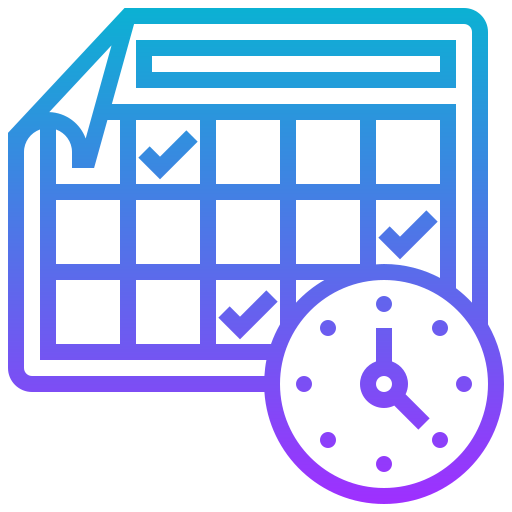
\includegraphics[width=2cm]{icono.png}
\end{center}
\end{figure}
\begin{Large}
\textbf{Agendaly} \\
\end{Large}
\begin{Med}
\textbf{Aplicación para la organización académica} \\
\end{Med}

\vspace*{3in}

\begin{large}
\raggedleft
\textbf{Autores:}Miguel Blanco Godón \\
Blanca Fernández Martín\\
Laura Cabezas González\\
\textbf{Fecha:}\textit{A Coruña, 16 de diciembre de 2021}\\
\end{large}

\end{center}
\end{titlepage} 

\newpage

\addtocontents{toc}{\hspace{-7.5mm} \textbf{Capítulos}}
\addtocontents{toc}{\hfill \textbf{Página} \par}
\addtocontents{toc}{\vspace{-2mm} \hspace{-7.5mm} \hrule \par}

\pagenumbering{empty}

\tableofcontents

\vspace{5cm}

\begin{flushright}
\begin{table}[hbtp]
\begin{center}

\caption{Tabla de versiones.}
\label{tabla:versiones}
\small
\vspace{1ex}

\begin{tabular}{|c|c|l|}
\hline
Versión & Fecha & Autor \\
\hline \hline
0.1 & 07/10/2021 & Grupo Q1.1 \\ \hline
0.2 & 09/11/2021 & Grupo Q1.1 \\ \hline
1.0 & 15/12/2021 & Grupo Q1.1 \\ \hline
x & y & \\ \hline
\end{tabular}

\end{center}
\end{table}
\end{flushright}


\newpage
\pagenumbering{arabic}


%%%%%%%
%%%%%%%
\section{Introducción}\label{cap.introduccion}

%%
\subsection{Objetivos}
El objetivo es la elaboración de una app de tipo agenda para organizar el estudio. Se podrán fijar fechas de entrega y exámenes de forma que se acceda a un calendario al que se puedan añadir eventos. También se podrá almacenar una copia del horario de clase en la aplicación, con información adicional de cada asignatura, como, por ejemplo, el aula en la que se imparte cada clase o el profesor. Se podrá entrar a la aplicación autenticándose mediante usuario y contraseña, y gracias a esto los usuarios registrados podrán organizarse en grupos, para sincronizar su forma de gestionar el estudio y repartir tareas entre ellos, de forma que cada miembro del grupo pueda marcar el estado en el que se encuentra la parte de la tarea en la que esta trabajando (si está trabajando todavía en ella, si está terminada, etc.) y el resto de integrantes puedan verlo. La aplicación también podrá acceder al reloj y podrá fijar recordatorios o alarmas en función de la hora, de forma que pueda avisar al usuario de que un día en concreto a partir de una hora determinada ha planeado que se tiene que poner a estudiar. Desde la aplicación también será posible compartir los documentos de los trabajos en grupo en la nube, y descargarlos para tener una copia y acceder a ellos sin conexión.
Se utilizará GitHub para el control de versiones de nuestra app. \cite{misc-git}
%%
\subsection{Motivación}
La buena gestión del tiempo es un aspecto básico para la consecución de un curso escolar. Por ese motivo necesitamos un mecanismo de gestión que nos ayude a mejorar nuestra producción académica con el menor esfuerzo posible, a través de un sistema sencillo, fácil de manejar, con control automático y centralizado que nos informe sobre los detalles de las diferentes tareas. 
Esta gestión se vuelve crítica cuando las tareas a realizar son grupales, especialmente si los integrantes tienen diferentes horarios. En este caso, un sistema de sincronización de tareas con recursos compartidos el cual monitorizase y notificara las tareas hechas y venideras a los diversos integrantes sería muy útil.
%%
\subsection{Trabajo relacionado}
Aplicaciones relacionadas con partes de nuestra app:
- TimeTune es una aplicación de gestión de tiempo y planificador de horarios \cite{misc-url1}

Reminder es una apps para recordatorios, alarmas y tareas. \cite{misc-url2}

Exam-countdown es una app para realizar un seguimiento de los exámenes y pruebas fechas.\cite{misc-url3}

Además también nos inspira mucho a la hora de saber las entregas la propia interfaz de moodle, ya que nos va indicando las entregas y su fecha límite.

%%%%%%%
%%%%%%%
\section{Análisis de requisitos}

%%
\subsection{Funcionalidades}
Las funcionalidades principales serán:
\begin{itemize}
\item \textbf{1.Fijar fechas en el calendario [feature/calendar]:} desde la aplicación habrá una forma de establecer citas que se crearán en un calendario. Se podrá fijar la fecha, el nombre del evento, y alguna nota informativa a mayores. La aplicación llevará una agenda donde se mostrarán ordenadamente los eventos creados y sus fechas.

\item \textbf{2.Almacenar el horario de clases [feature/horario]:} se podrá crear un horario semanal introduciendo las asignaturas y algún atributo a mayores, por ejemplo, el aula en la que se imparte y la hora . El horario será visible nada más abrir la aplicación.

\item \textbf{3.Autenticación[feature/authentication]:} el usuario podrá identificarse al entrar en la app, de forma que pueda acceder a sus datos desde otros dispositivos. Además, la autenticación del usuario verifica su identidad frente a otros usuarios a la hora de trabajar en grupos.

\item \textbf{4.Notificaciones de estudio[feature/notification]:} el usuario podrá fijar el tiempo diario que le quiera dedicar a cada tarea y organizarlo en el día. La aplicación almacenará esta información y emitirá notificaciones a las horas establecidas a modo de recordatorio.


\end{itemize}

Y las funcionalidades secundarias serán:
\begin{itemize}

\item \textbf{Grupos de trabajo:} se podrán establecer tareas conjuntas para los integrantes de un grupo, y cada integrante podrá ir actualizando el avance de su trabajo de forma pública para el resto de sus compañeros.

\item \textbf{Apuntes en la nube:} el usuario podrá acceder a archivos que hayan compartido otros usuarios de a los que pertenezca. Será posible descargar estos documentos para poder acceder sin conexión. 
\end{itemize}

%%
\subsection{Prioridades}
El objetivo principal de esta aplicación es implementar de forma simple las funcionalidades de una agenda, aprovechando las comodidades que puede aportar un telefono movil. Es por esto que las prioridades serán las tareas más cercanas a la funcionalidad de la agenda, es decir, fijar las fechas de los eventos importantes en un calendario, mostrar los eventos proximos, mantener una copia facilmente accesible del horario semanal y el sistema de notificaciones para el estudio diario. 



%%%%%%%
%%%%%%%
\section{Planificación inicial}

%%
\subsection{Iteraciones}
Se harían cuatro iteraciones incrementales. En la primera, se intentará que la aplicación tenga su funcionalidad básica: horario, gestión de calendario y usuarios.
En la segunda iteración se haría la extensión multiusuario y notificación: notificaciones, creación de grupos y sincronización básica de tareas. También se corregirían errores de la iteración anterior.
En la tercera iteración se añadirá el repositorio de datos común y la gestión comunal de tareas. También se corregirán los errores de la iteración anterior.
En la iteración final, se corregirán los fallos de las iteraciones anteriores y se hará la integración final de conjunto.

%%
\subsection{Responsabilidades}
Se llevará a cabo la implementación de tres funcionalidades simultaneamente, para que todos los miembros del grupo puedan trabajar simultaneamente sin tener que esperar a por el trabajo de los demás. Las primeras funcionalidades a implementar se repartirán tal que 
la creación eventos en el calendario será implementada por Blanca Fernandez, el horario semanal por Laura Cabezas y la autenticación por Miguel Blanco. 
\newline
La creación y gestión de equipos será responsabilidad de Miguel Blanco. El añadir notificaciones al horario será responsabilidad de Laura Cabezas.Y añadir notificaciones al calendario será responsabilidad de Blanca Fernandez.
%%
\subsection{Hitos}
Se realizará una entrega por cada funcionalidad implementada, más otras dos a mayores, al final de cada iteración, donde se solucionarán los detalles de integración de las partes en las que se dividió el trabajo. Por lo tanto, habrá tres hitos iniciales para las tres funcionalidades ya repartidas, y un cuarto hito donde se mostrará una primera versión funcional de la aplicación, aunque con funcionalidades reducidas. Más adelante, volverá a haber un hito por cada funcionalidad secundaria que se implemente, y finalmente, la entrega final de la aplicación completa.
En cuanto a los test, en cada hito de una funcionalidad aislada se creará un test para esa funcionalidad, y para el hito que compruebe la integración de las partes, un test común para las funcionalidades que estén implementadas hasta ese momento.
%%
\subsection{Incidencias}
Debido a la forma en la que se va a desarollar el proyecto y estar divido en pequeñas funcionalidades que se desarrollarán independientemente, la cohesión de las partes puede llegar a ser un punto crítico.
Un riesgo a tener en cuenta a la hora del diseño es el uso de repositorios externos, ya que si no lo controlamos podemos perder funcionalidades. \cite{misc-hc}

Se completará esta sección cuando se haya llegado a un grano suficientemente fino en la planificación del proyecto y se conozcan más detalles sobre la implementación.
Cuando estos detalles sean conocidos se clasificarán las posibles incidencias segun su gravedad y se poporcionará una solución acorde. Los diferentes grados serán incidencias leves (bugs), incidencias de grado medio (fallo en una funcionalidad/caso de uso), o incidencias graves (a nivel de toda la aplicación/arquitectura/caso de uso no satisfacible).

%%%%%%%
%%%%%%%
\section{Diseño}

%%
\subsection{Arquitectura}
Para esta aplicación vamos a usar el patrón de arquitectura Clean.

\subsection{Persistencia}
Para la persistencia de usuarios se utilizarán ficheros de shared preferences almacenados en local. Por seguridad, las contraseñas estarán cifradas. Los eventos de calendario/horario se guaradarán en una base de datos de Firebase. Para guardar los datos usaremos dos bases de datos implementadas con Room, una para el calendario y otra para el horario.

\subsection{Vista}
Ver figuras 1,2, y 3.
\begin{figure}
            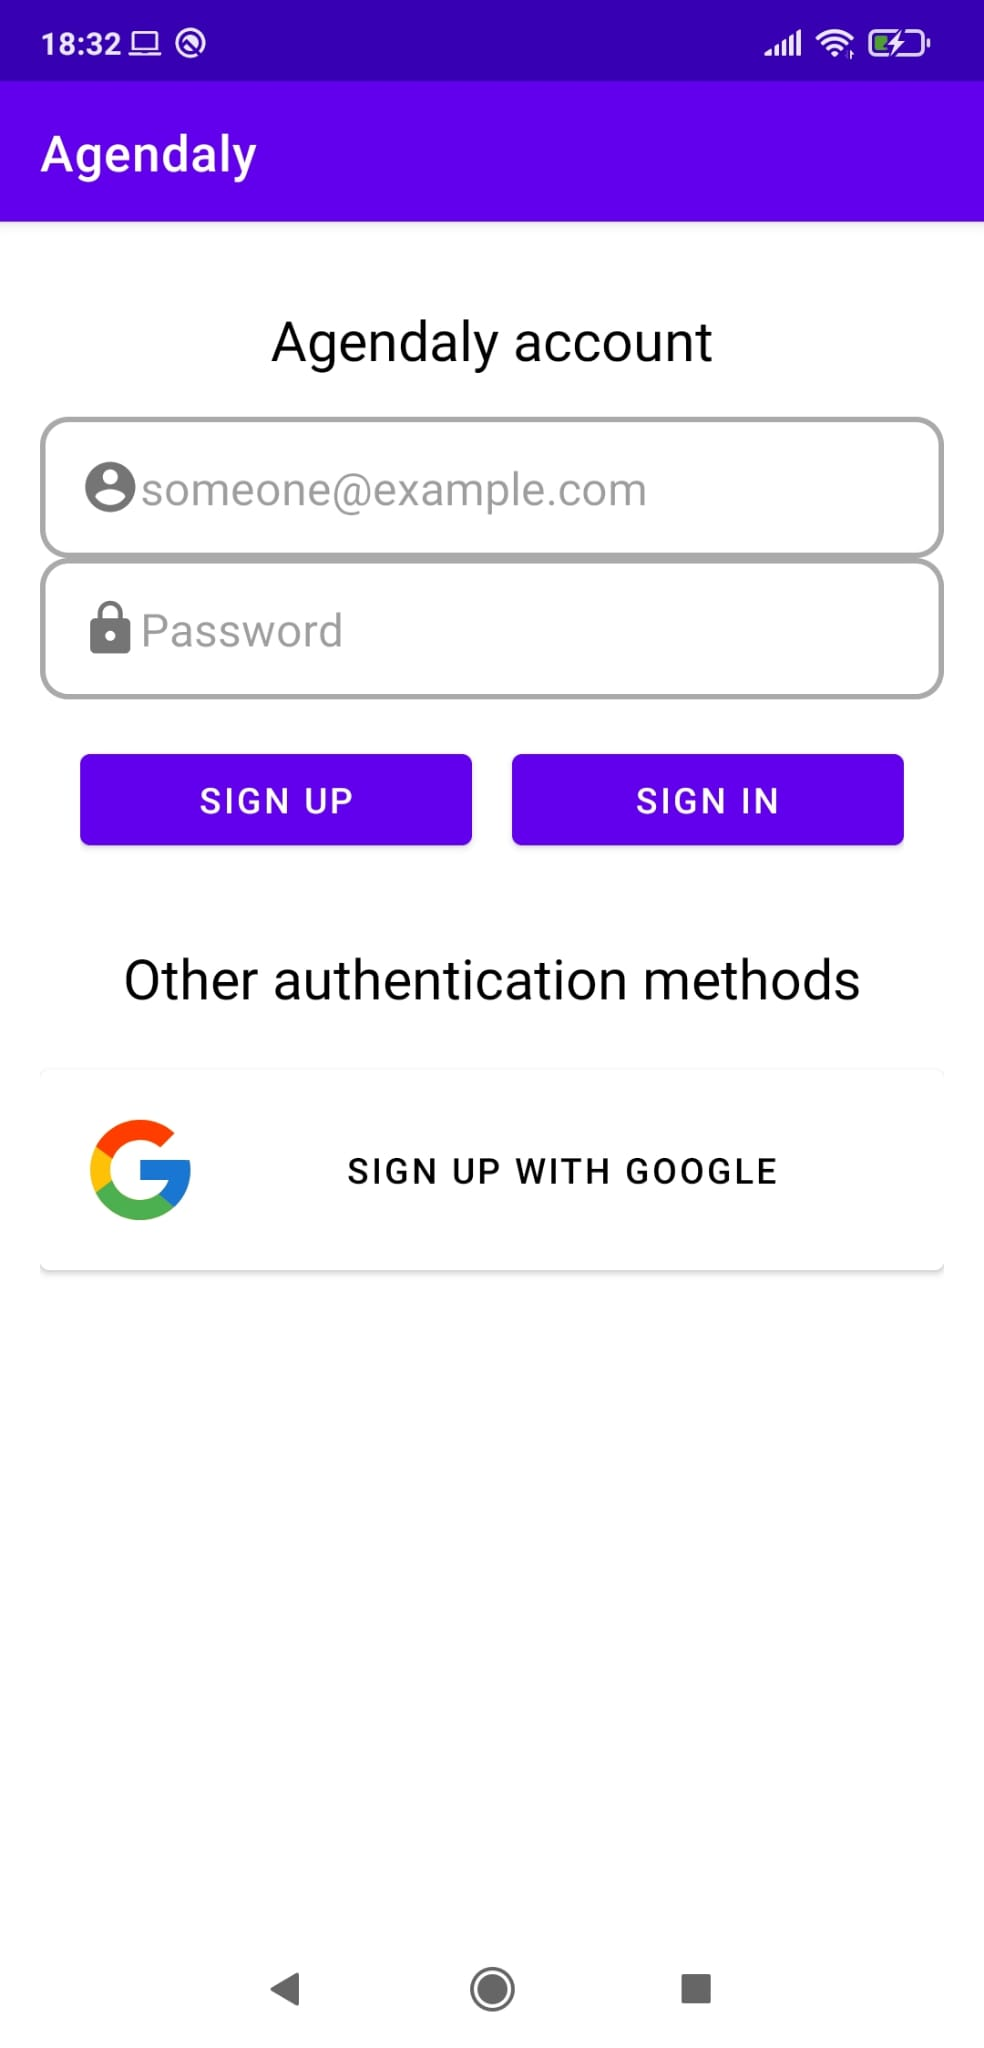
\includegraphics[scale=0.05]{view.jpeg} \hfill
            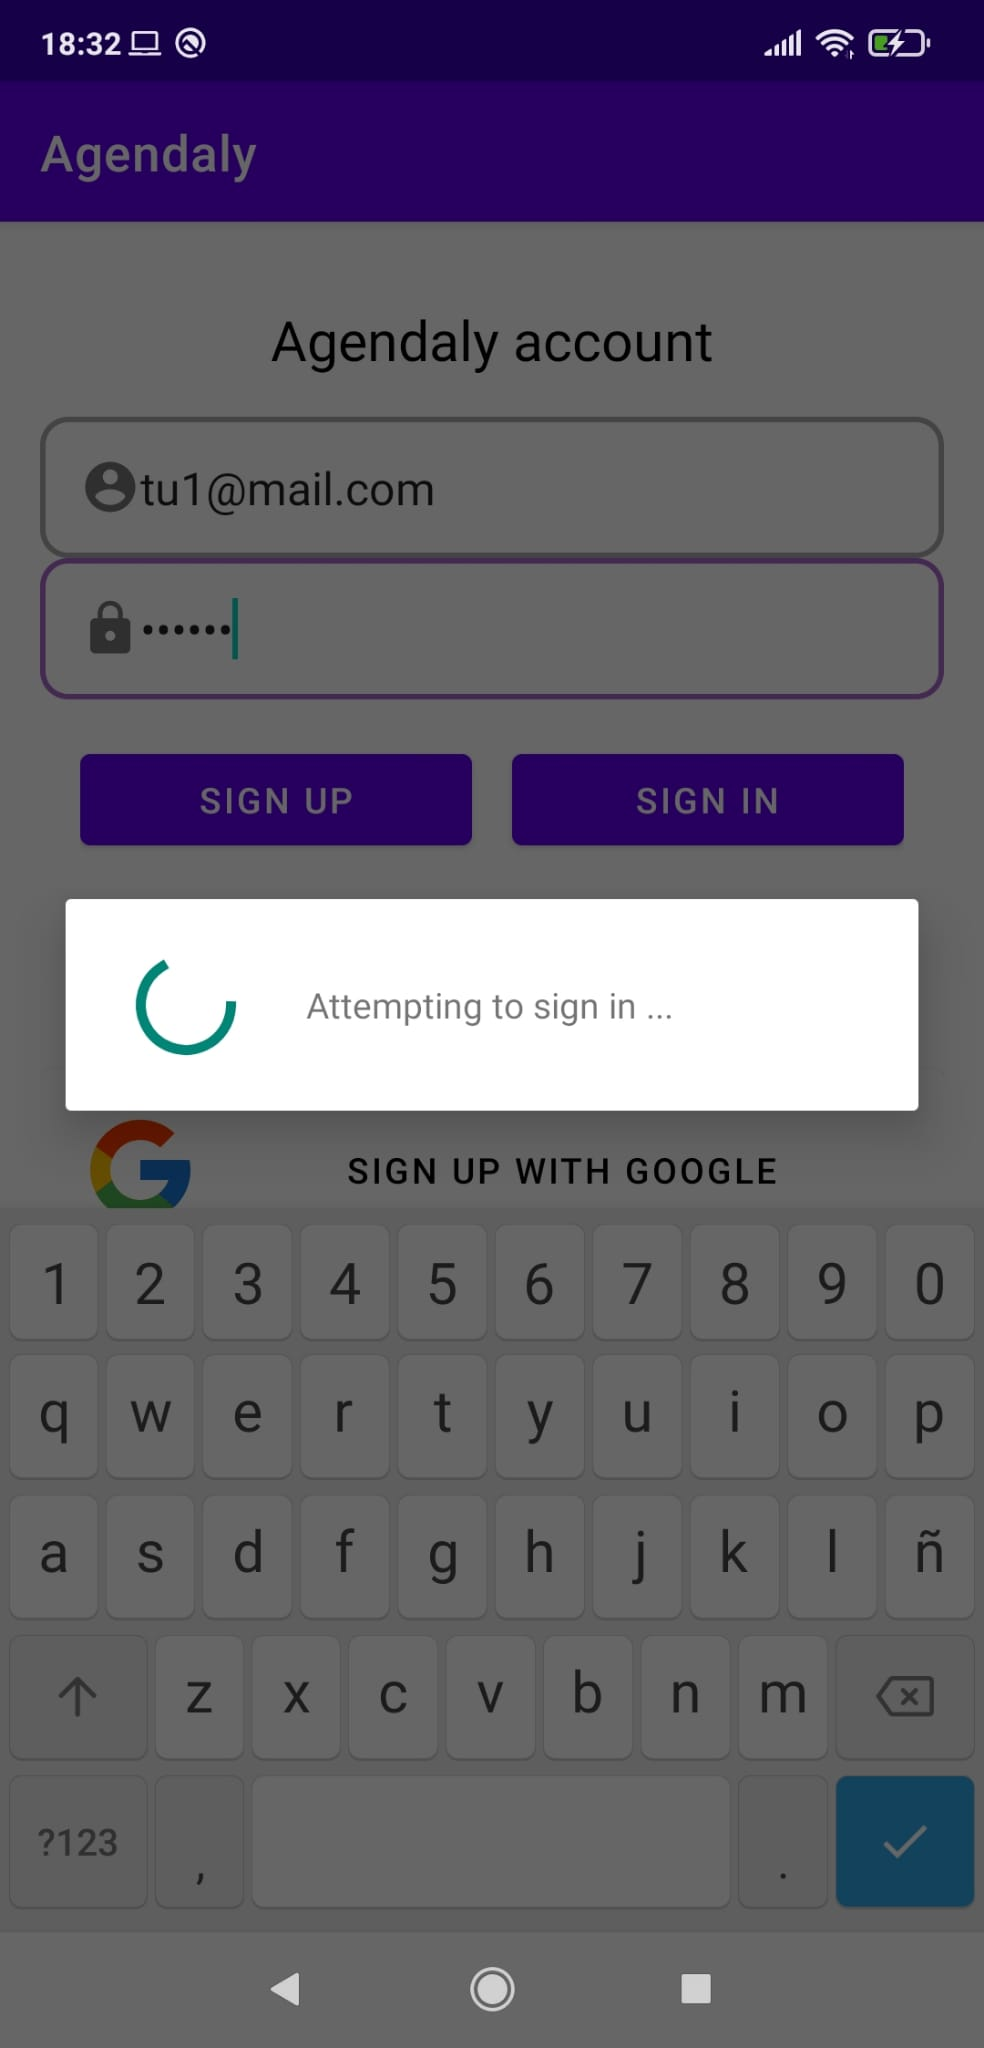
\includegraphics[scale=0.05]{dialog.jpeg}\hfill
            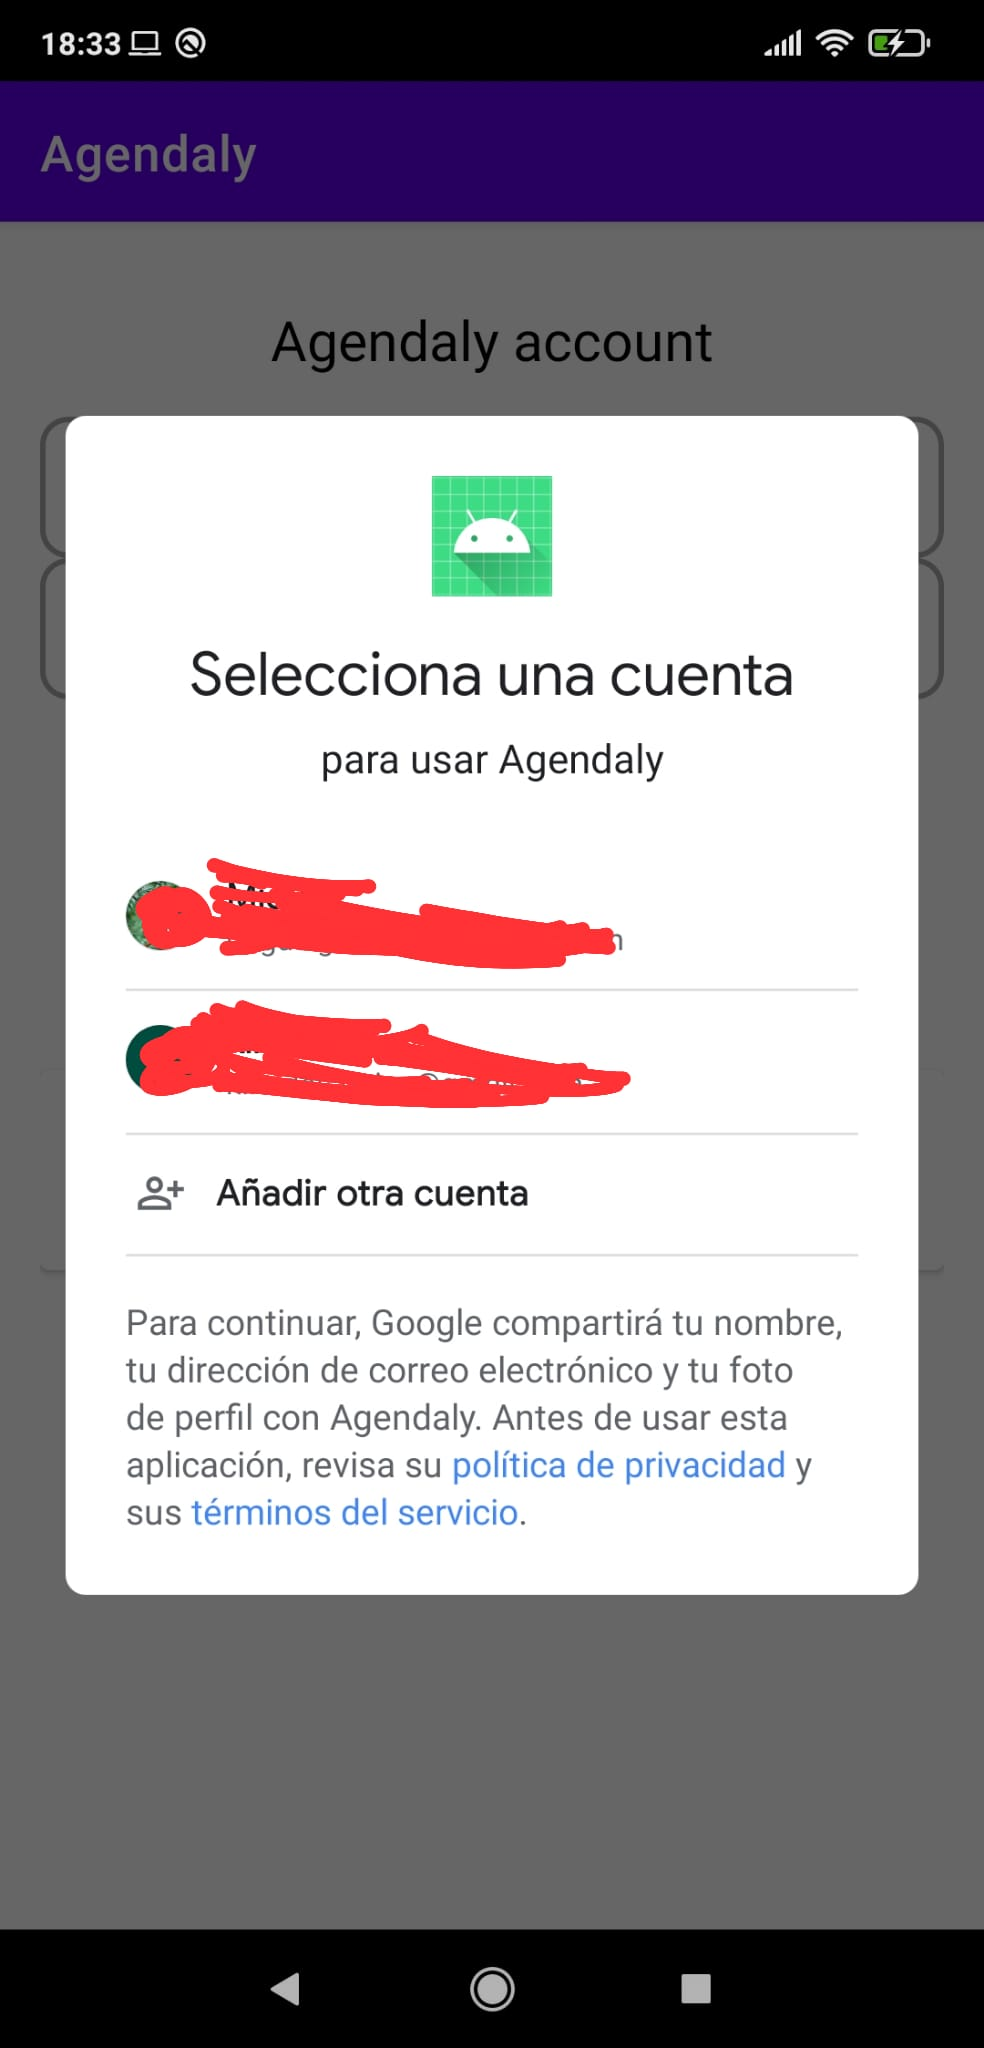
\includegraphics[scale=0.05]{google.jpeg} \hfill
            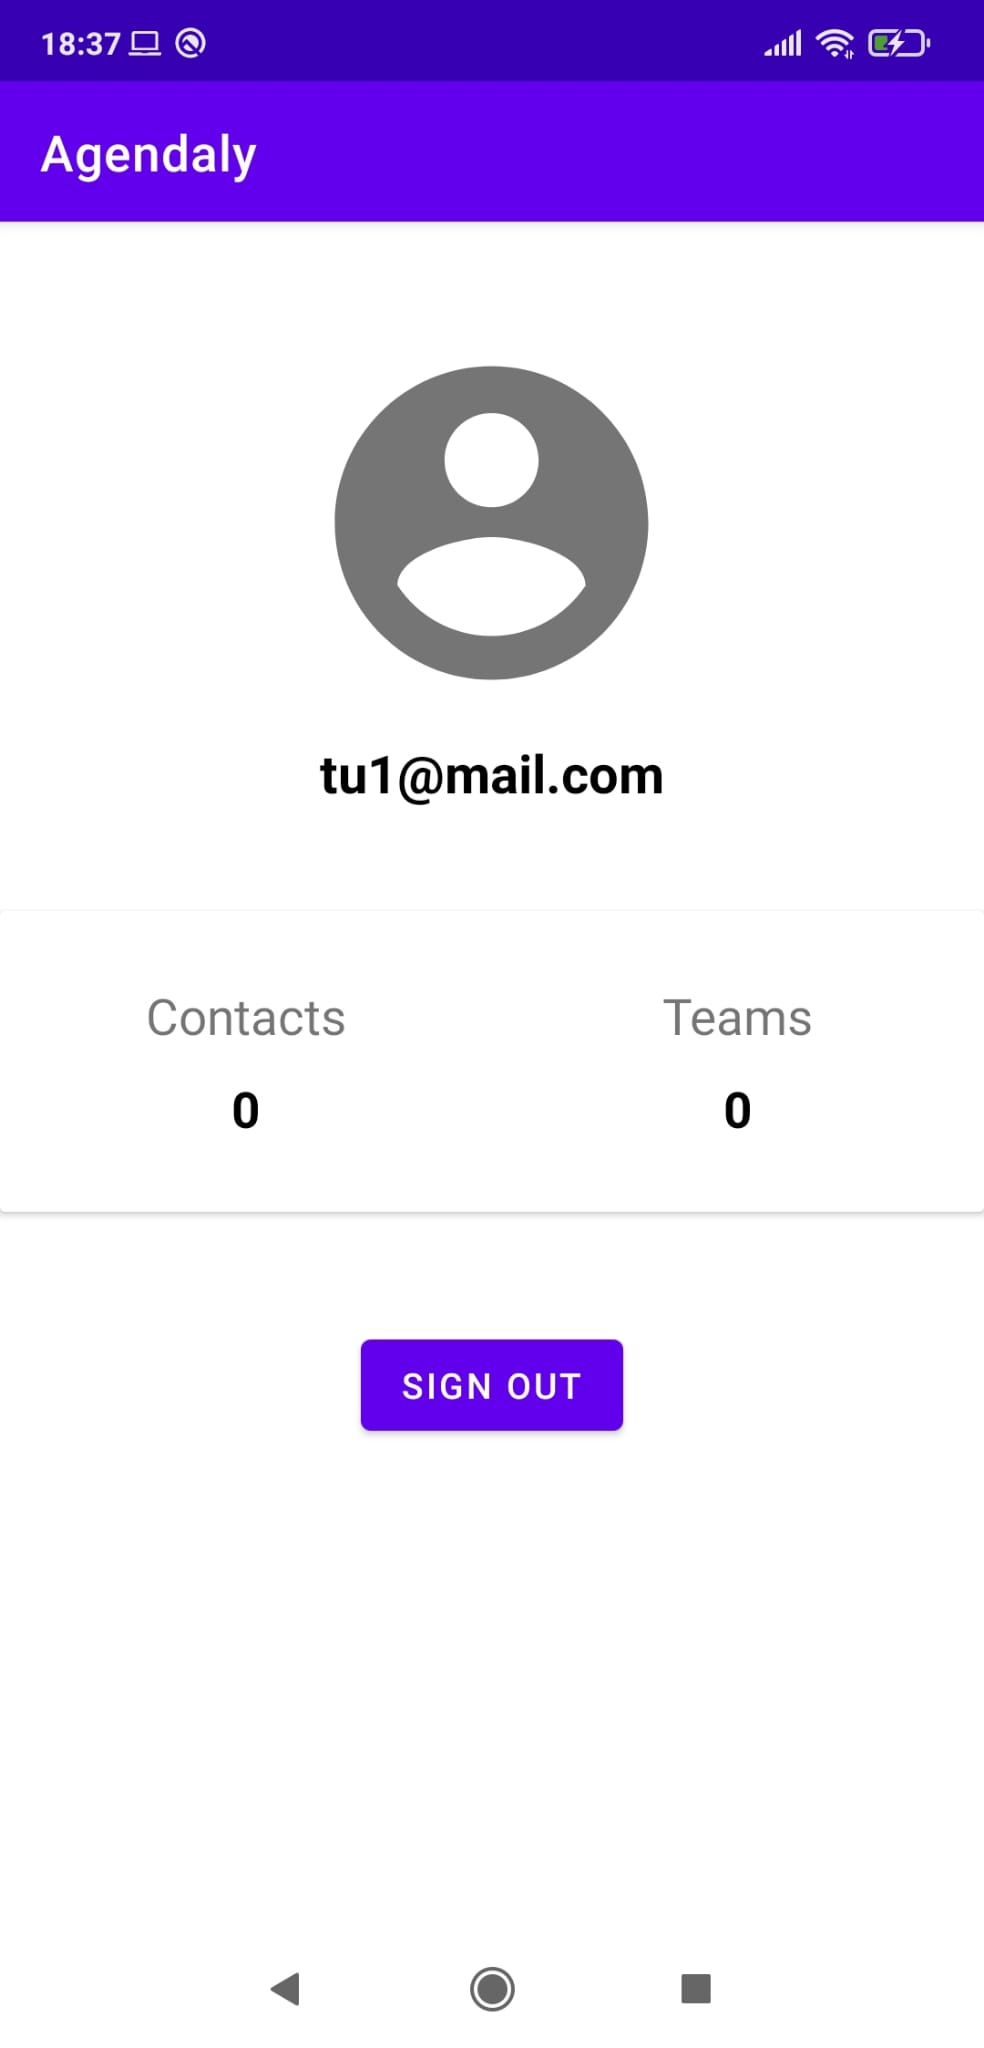
\includegraphics[scale=0.05]{account_view.jpeg}
            \caption{Pantallas de autenticación}
        \end{figure}
        
\begin{figure}
            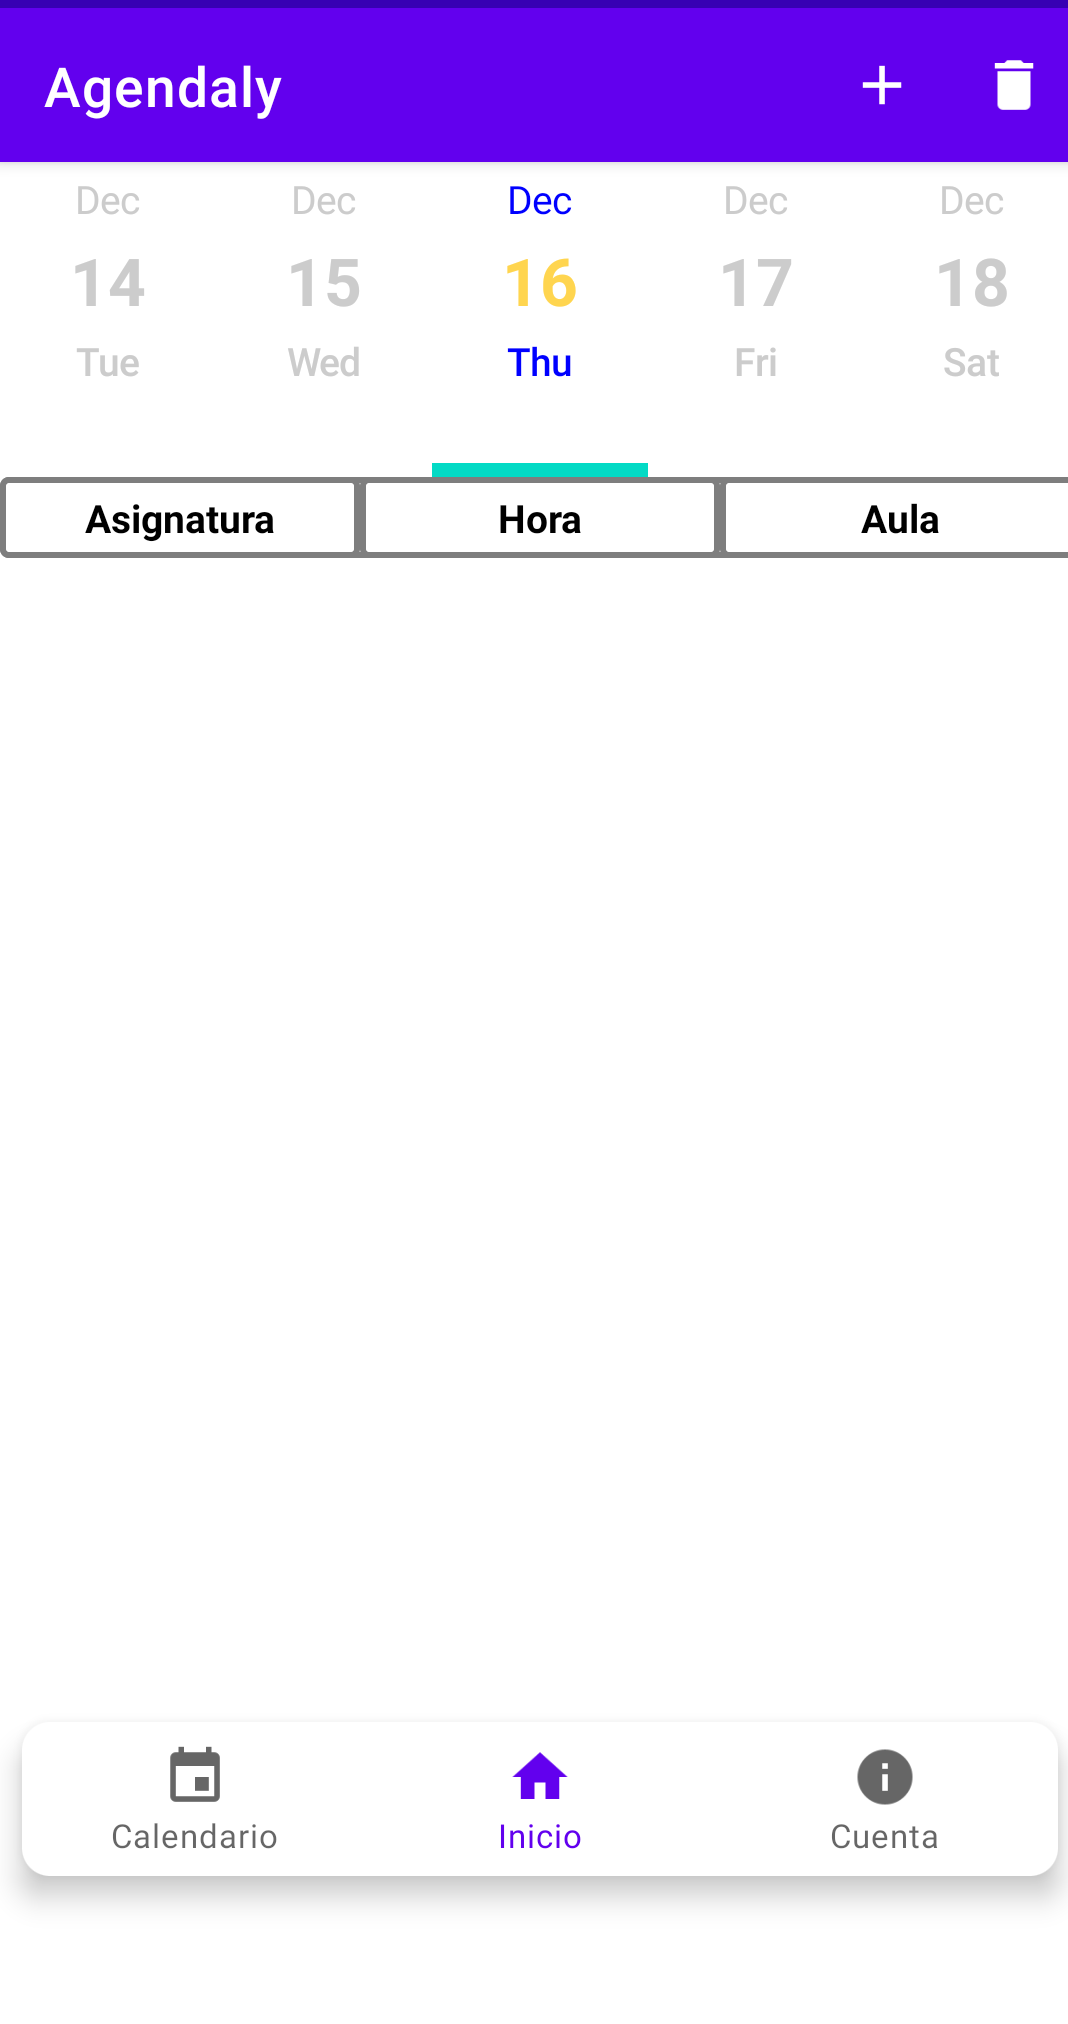
\includegraphics[scale=0.05]{Horario.png} 
            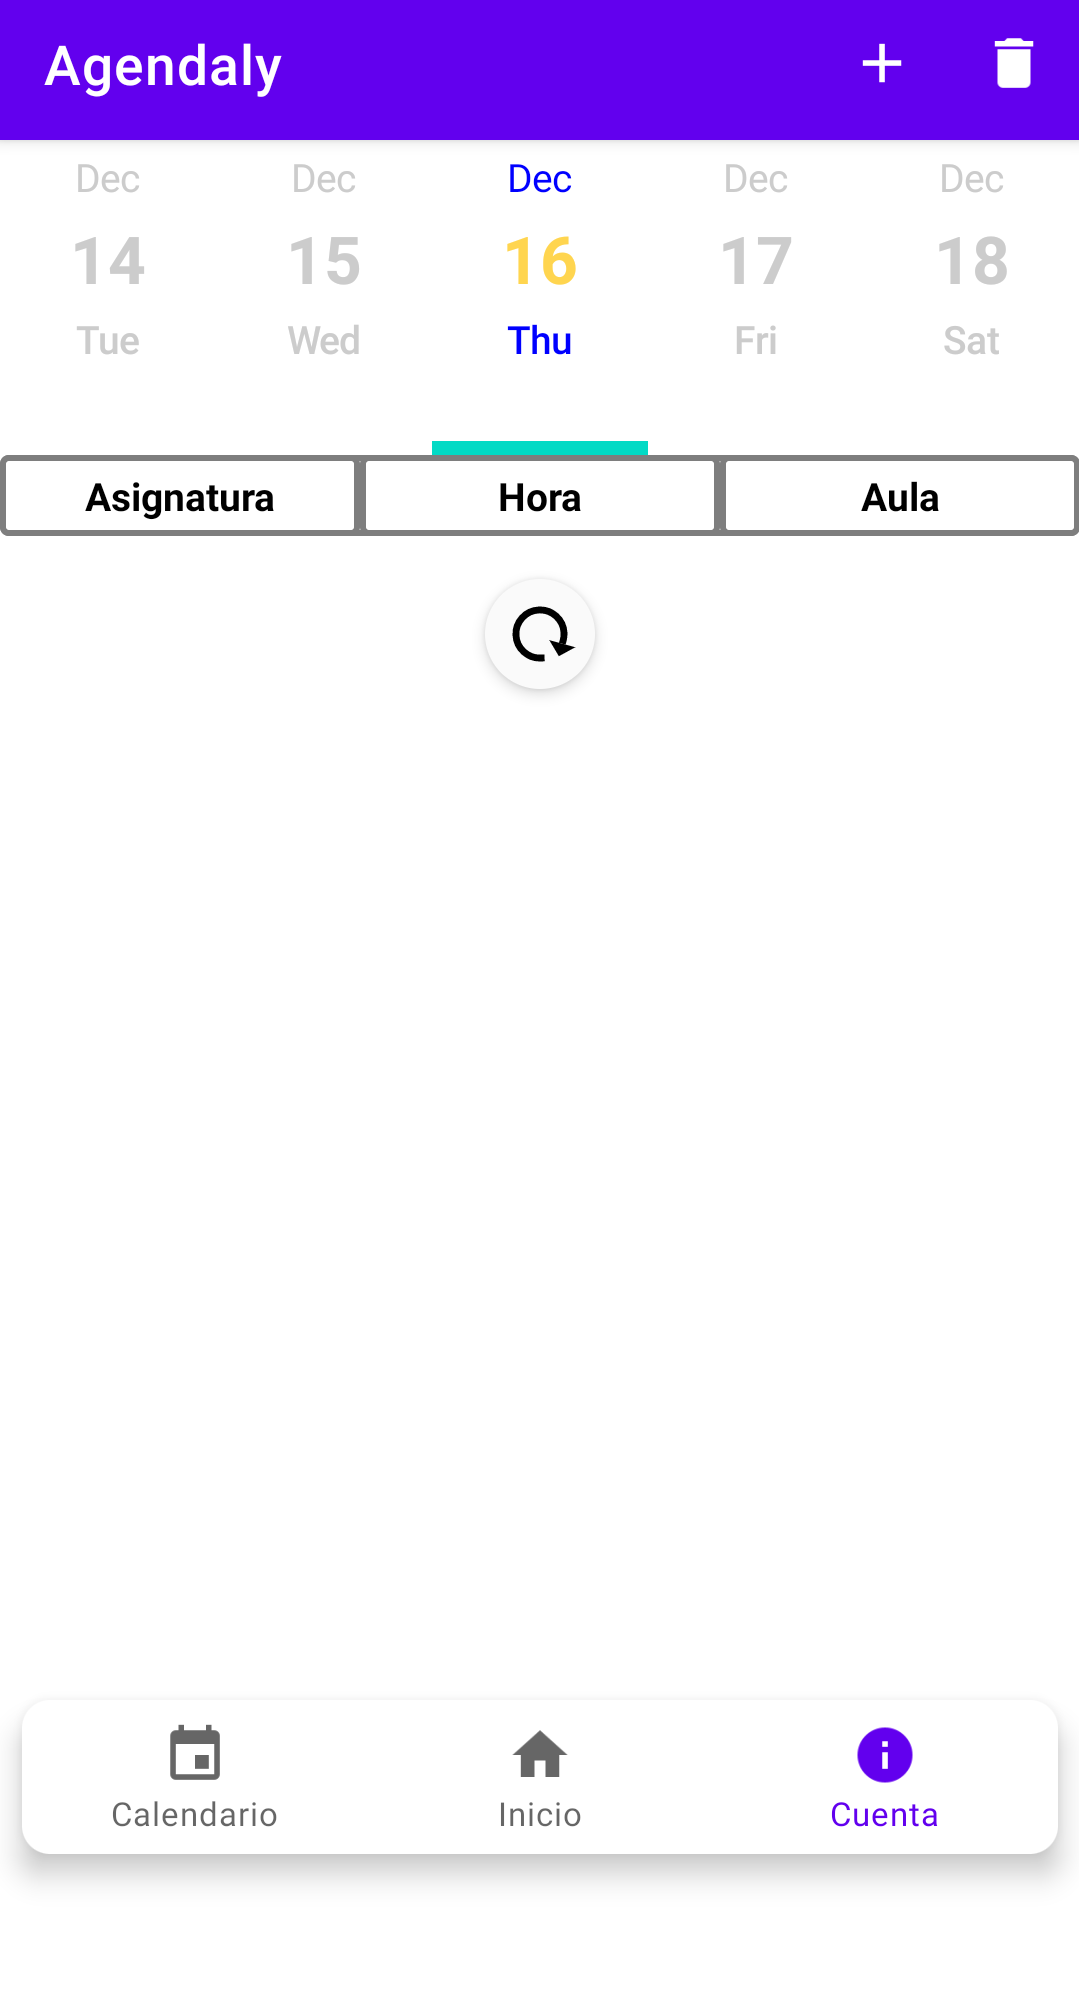
\includegraphics[scale=0.05]{swipe.png}\hfill
            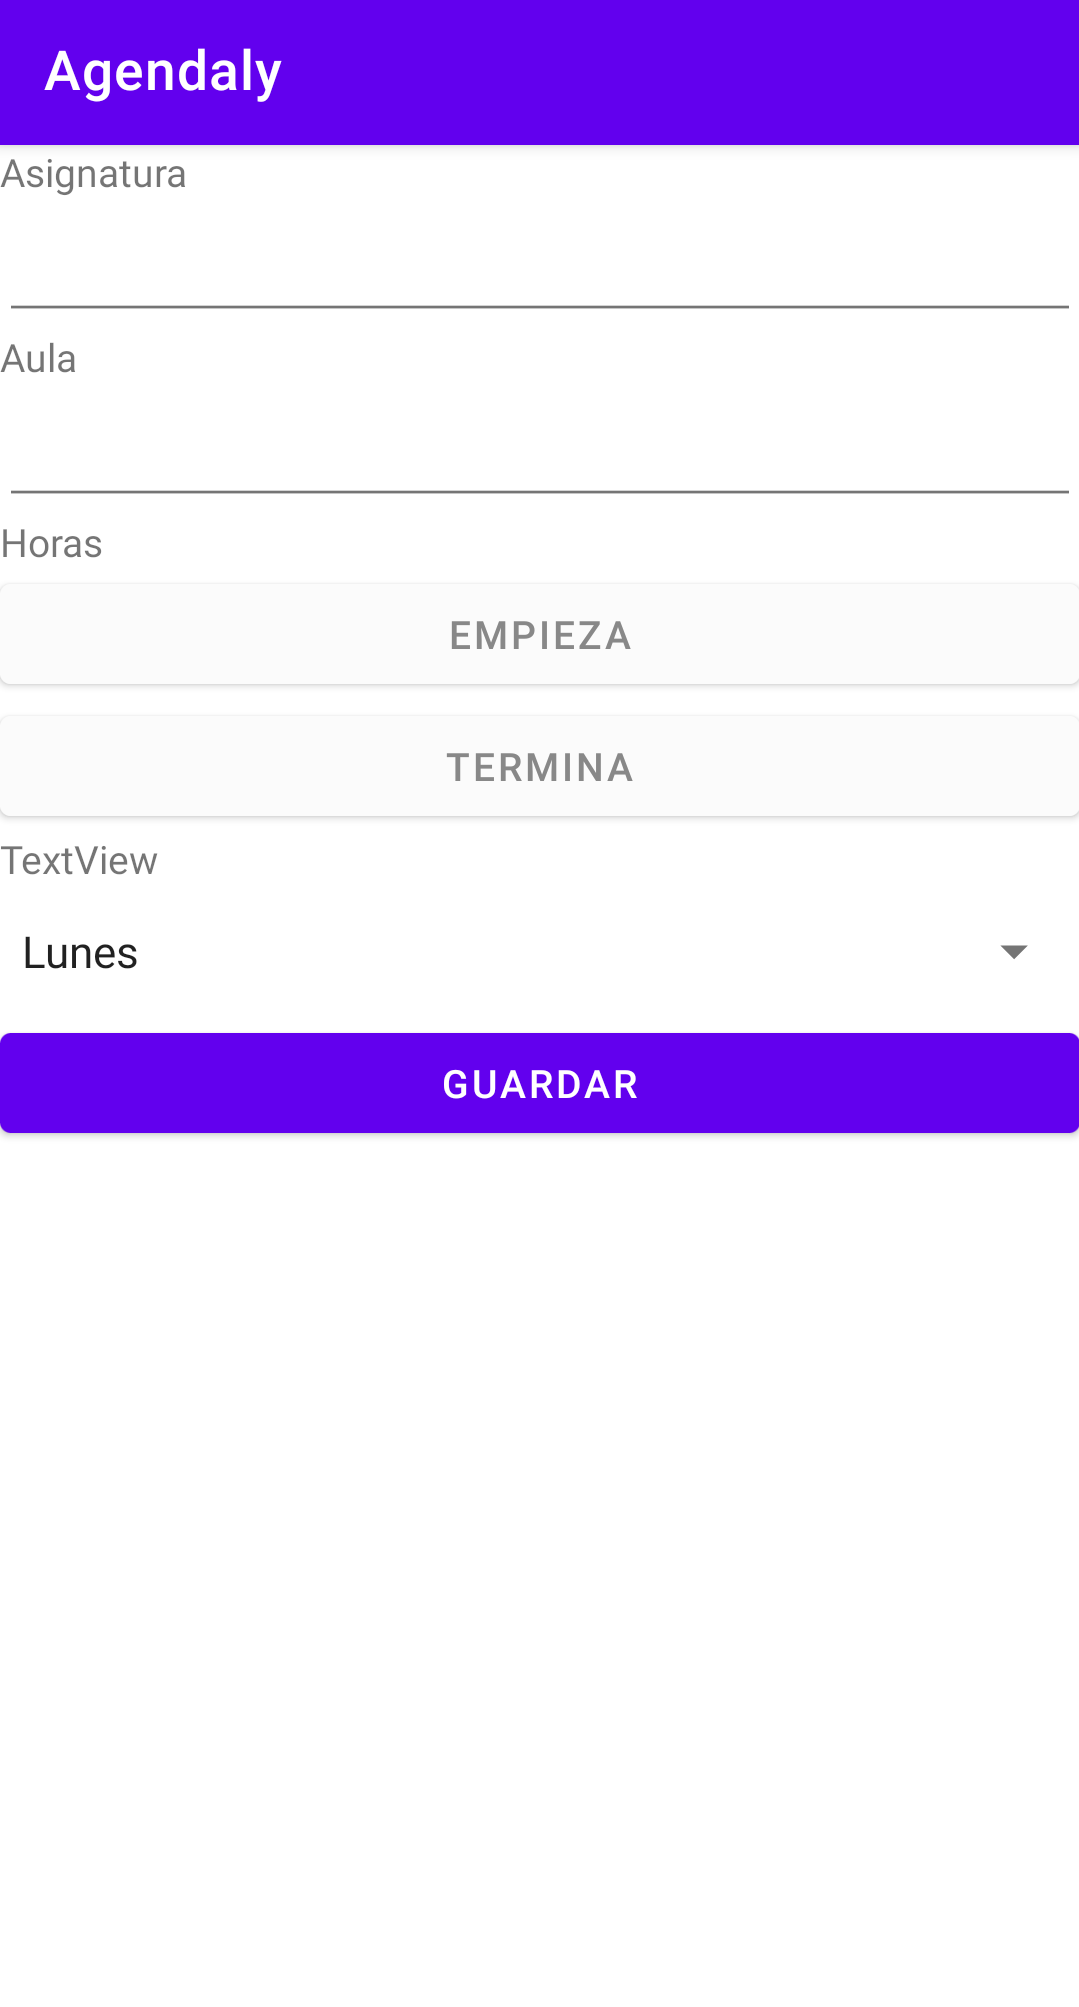
\includegraphics[scale=0.05]{Add.png} 
            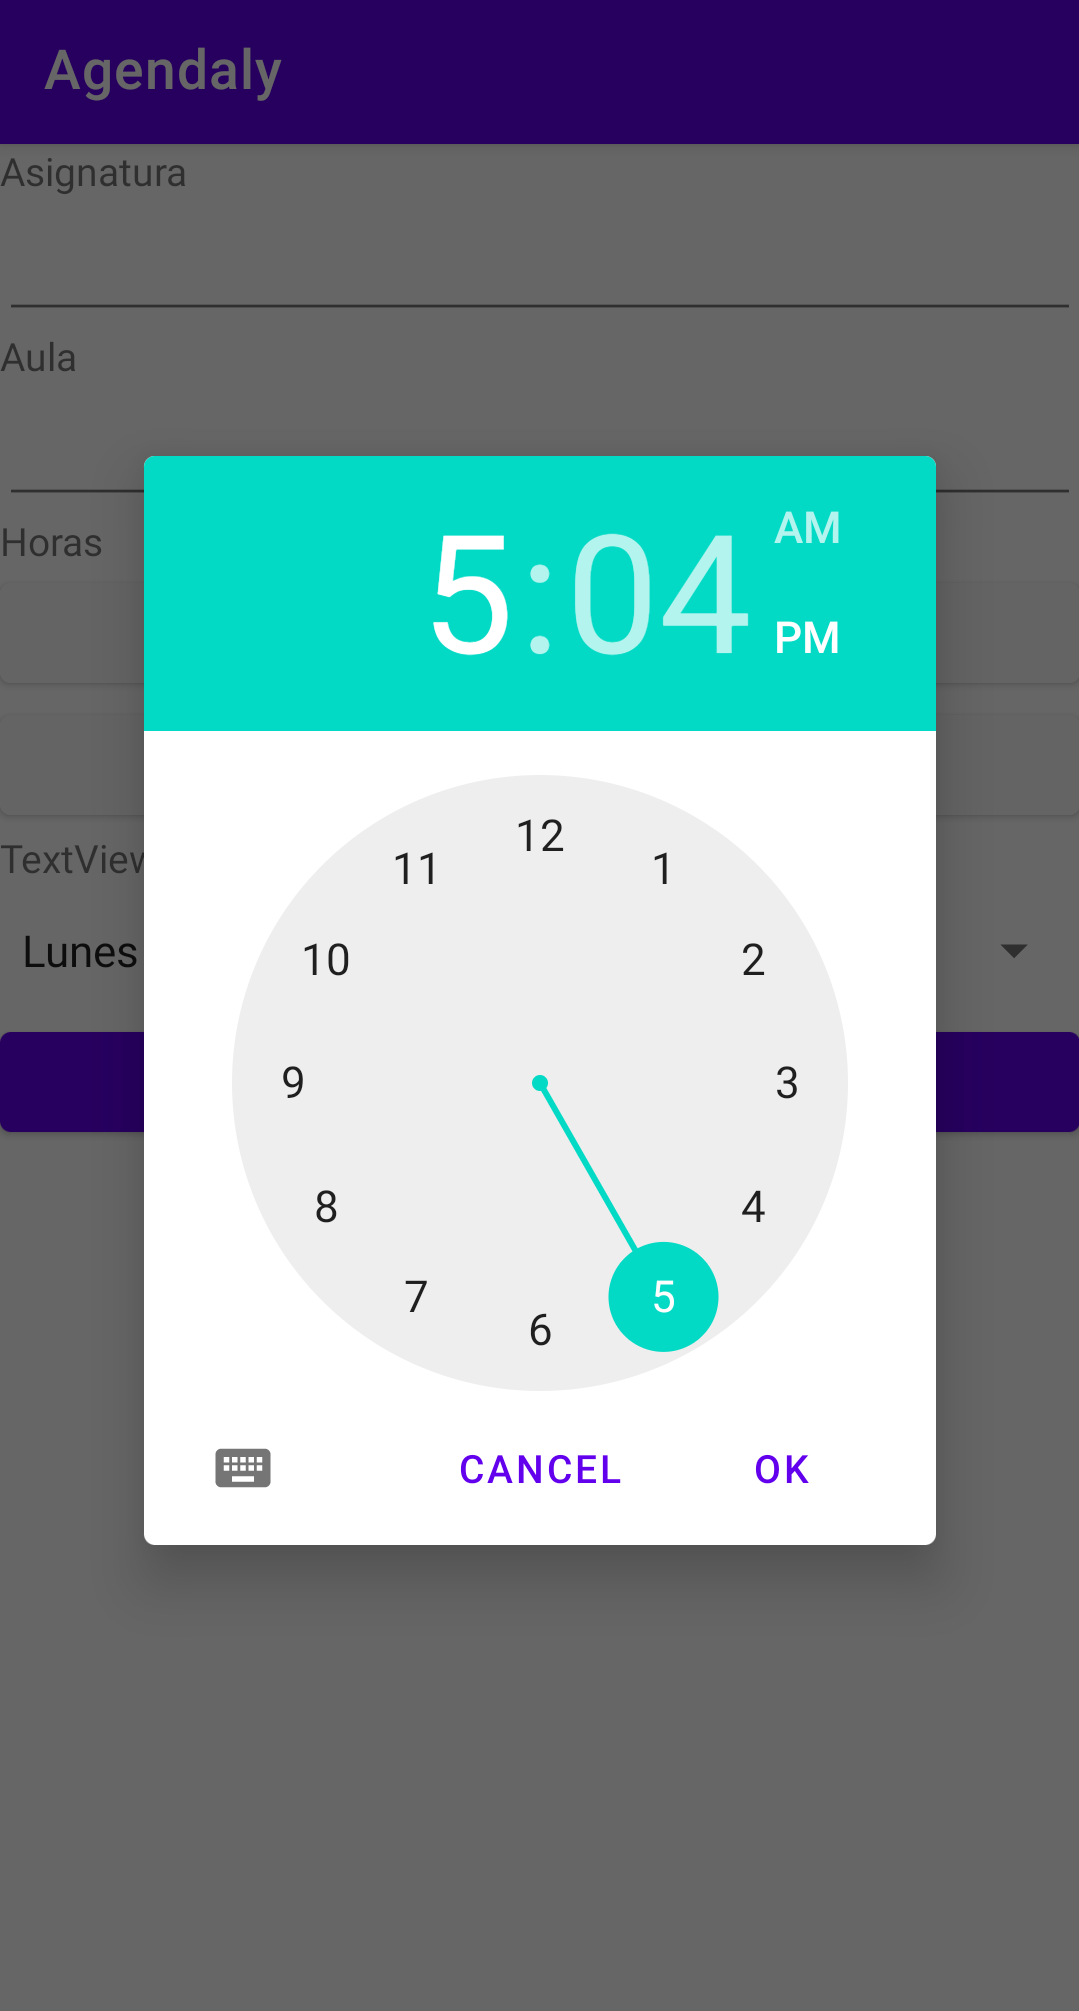
\includegraphics[scale=0.05]{add_timepicker.png}
            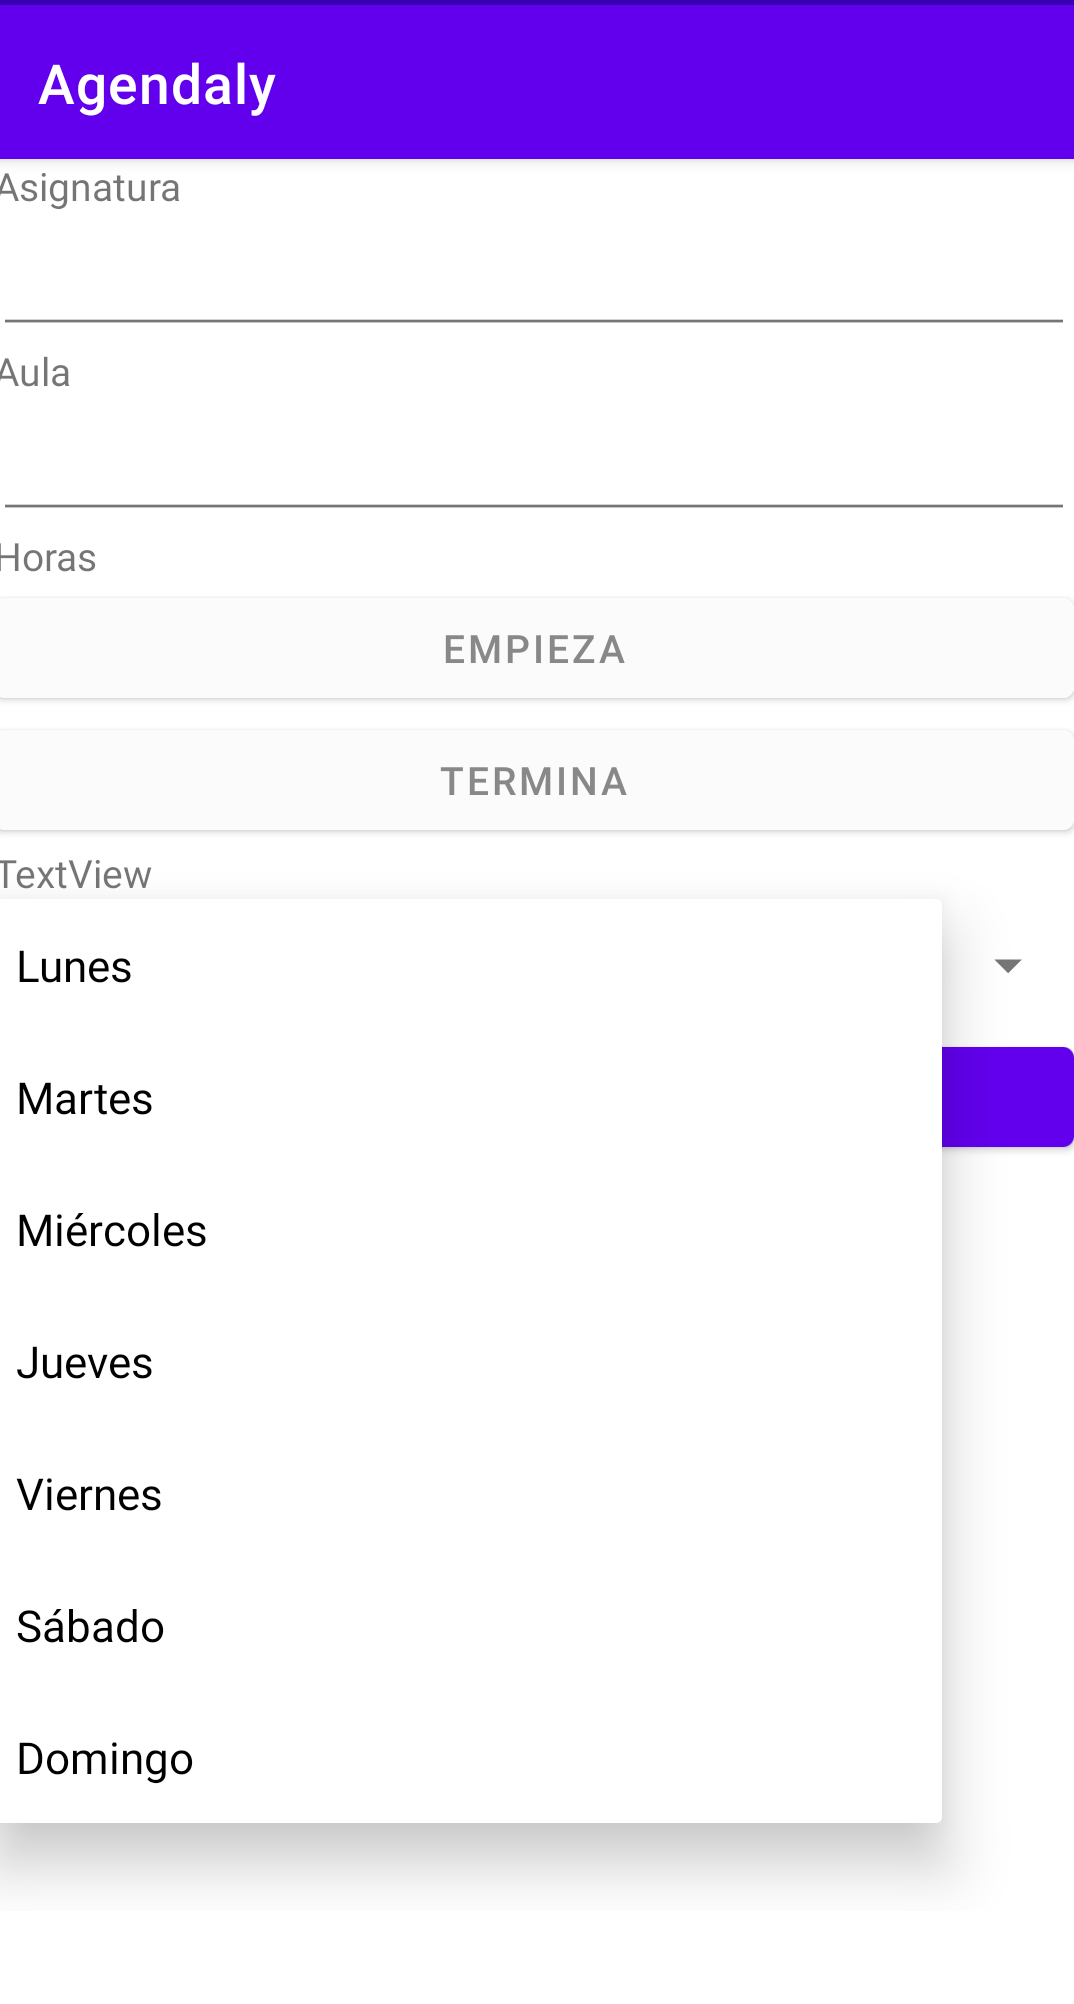
\includegraphics[scale=0.05]{add_spinner.png}
            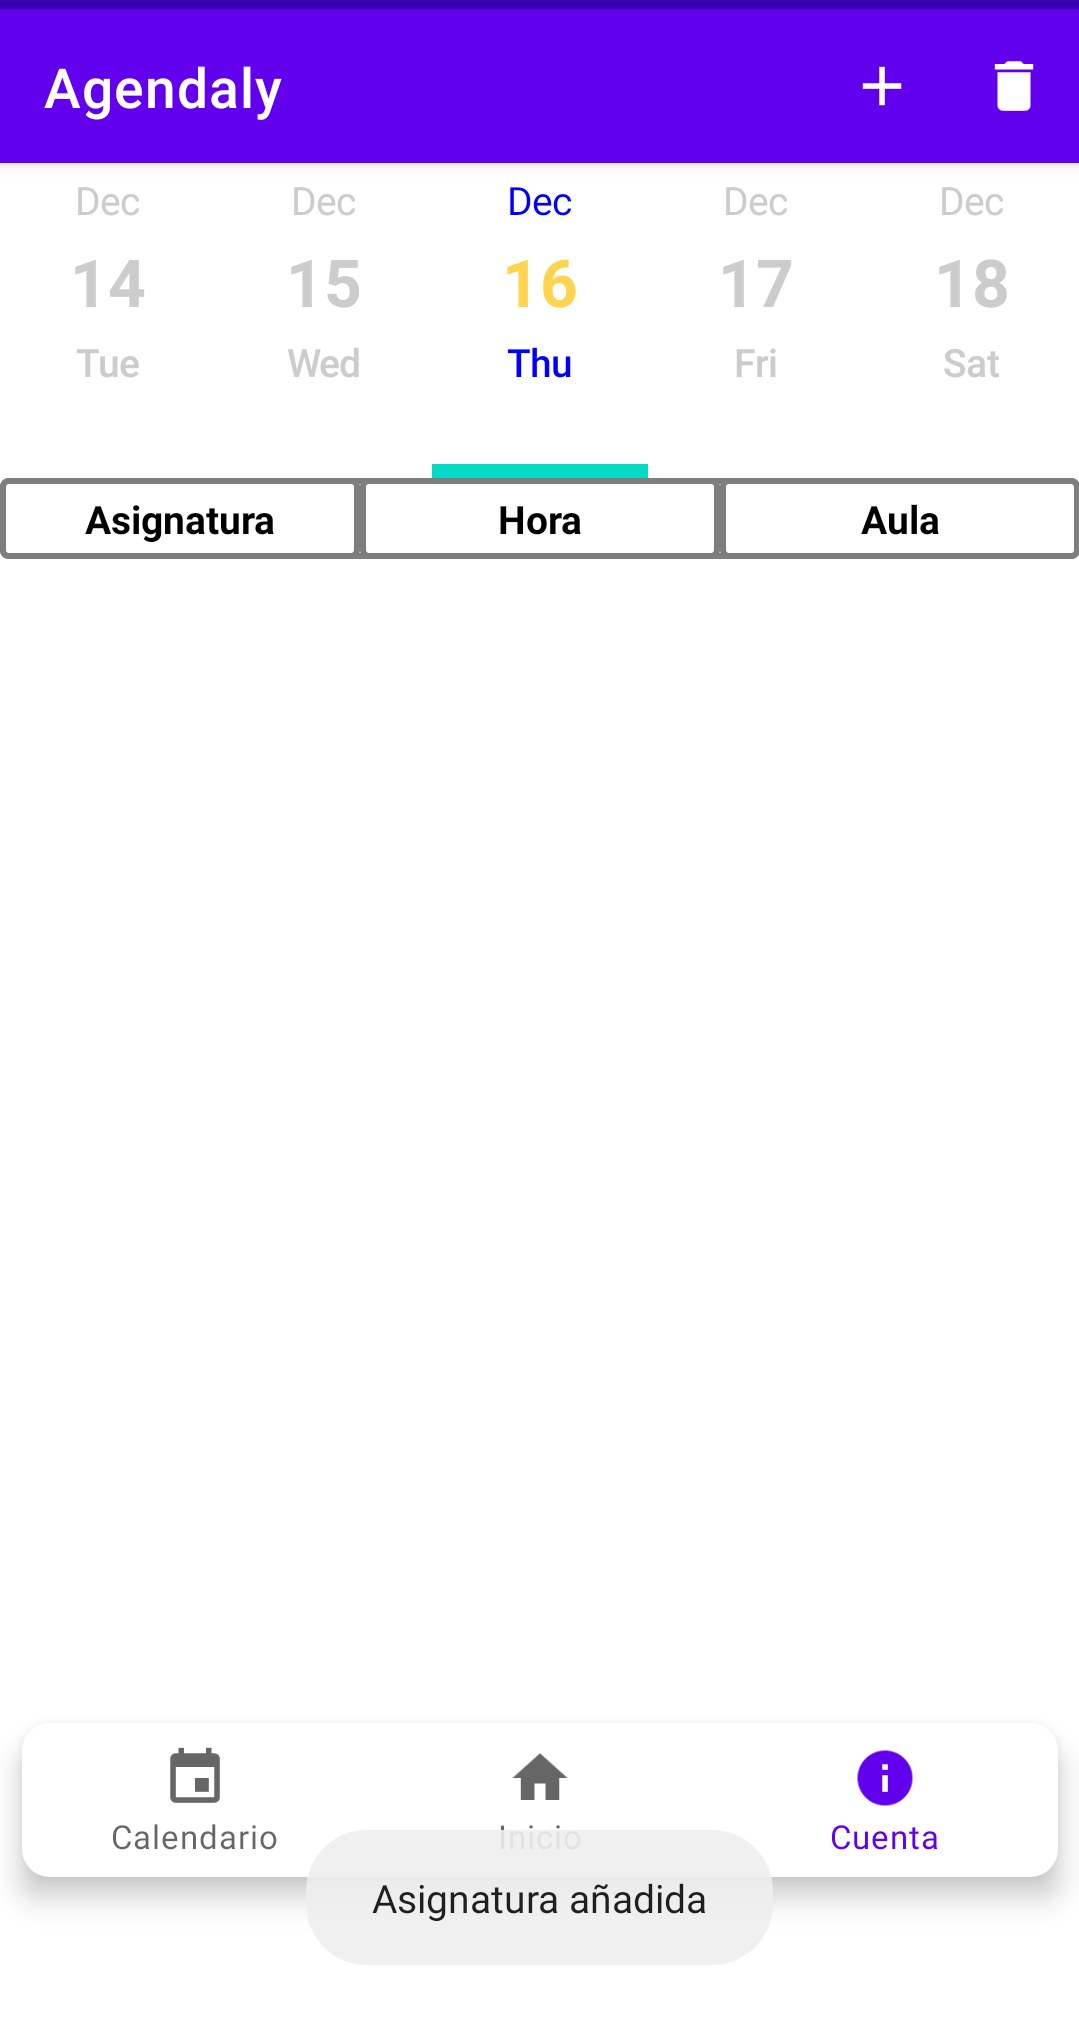
\includegraphics[scale=0.05]{ToastAdd.png}\hfill
            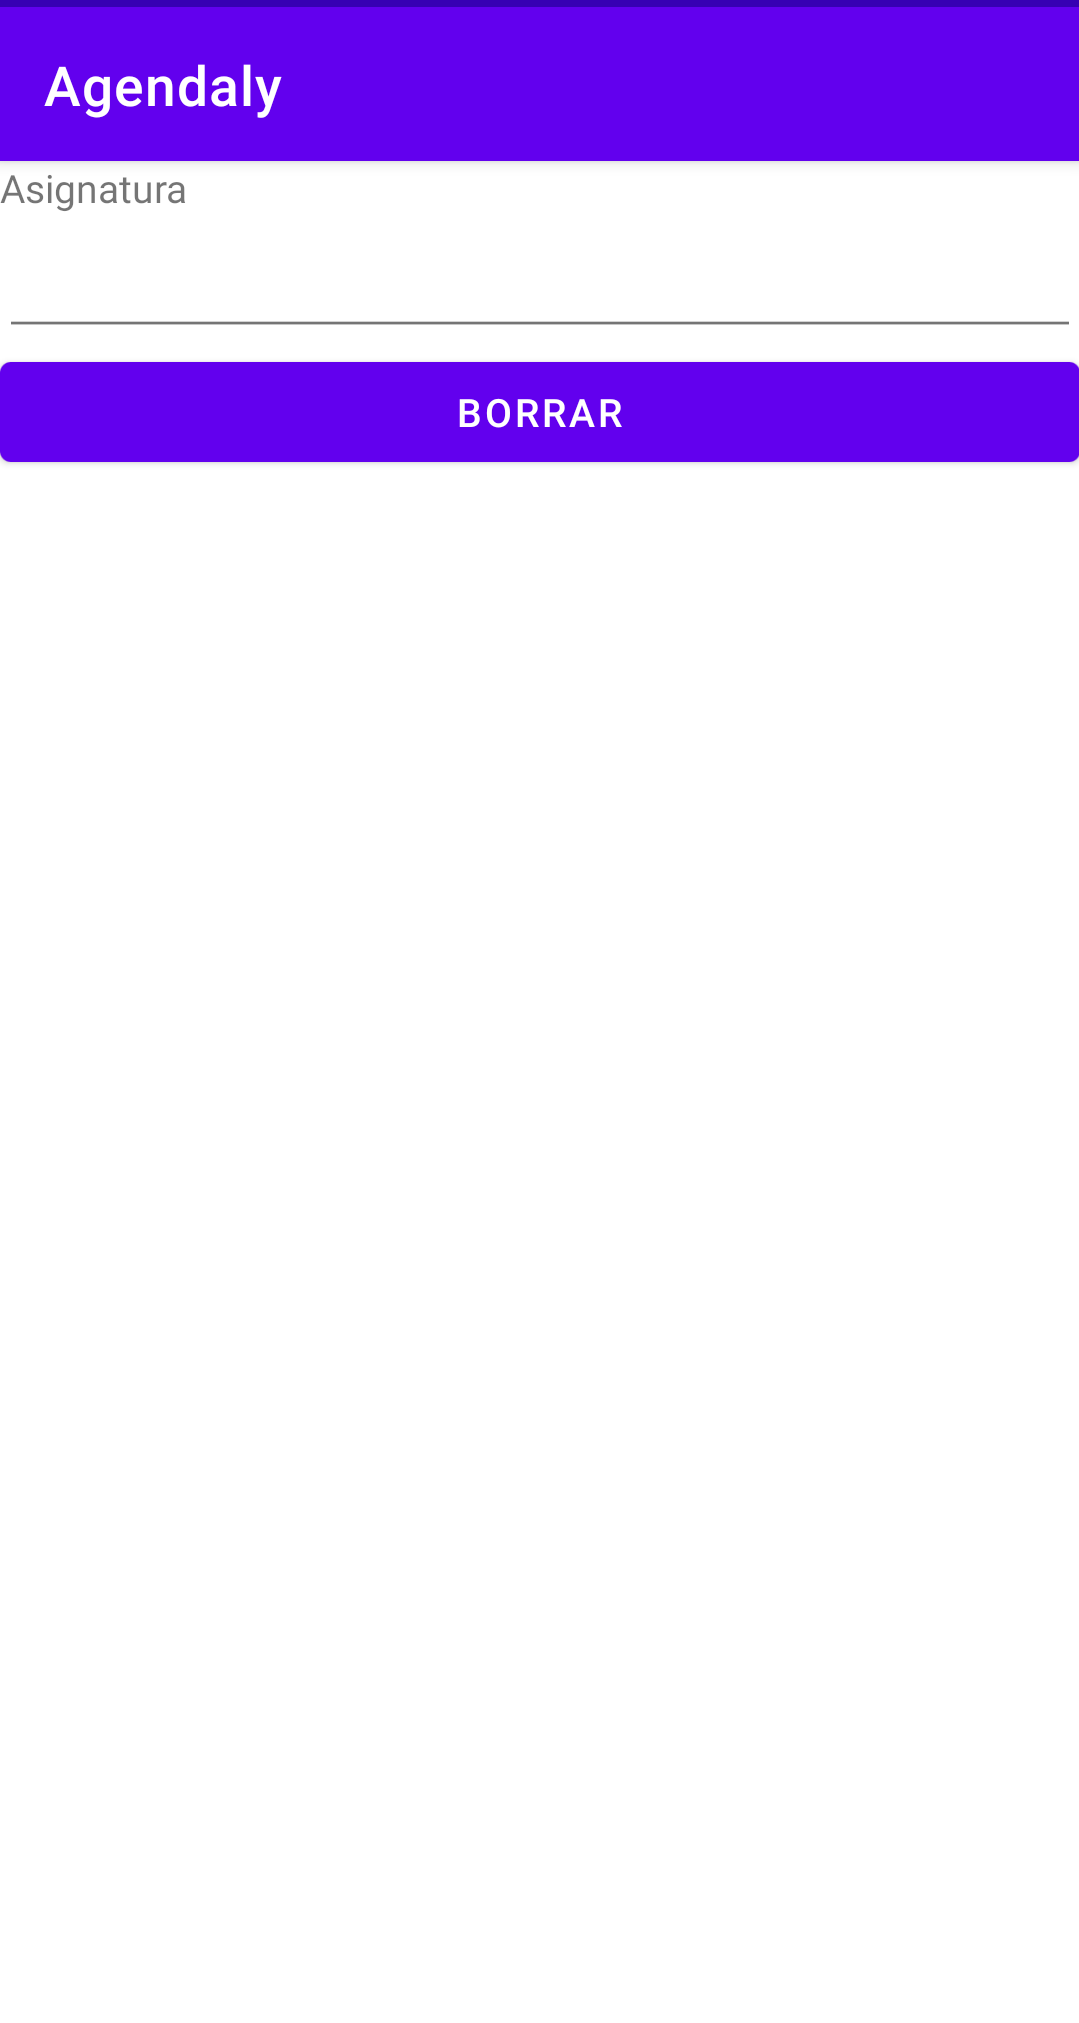
\includegraphics[scale=0.05]{borrar.png}
             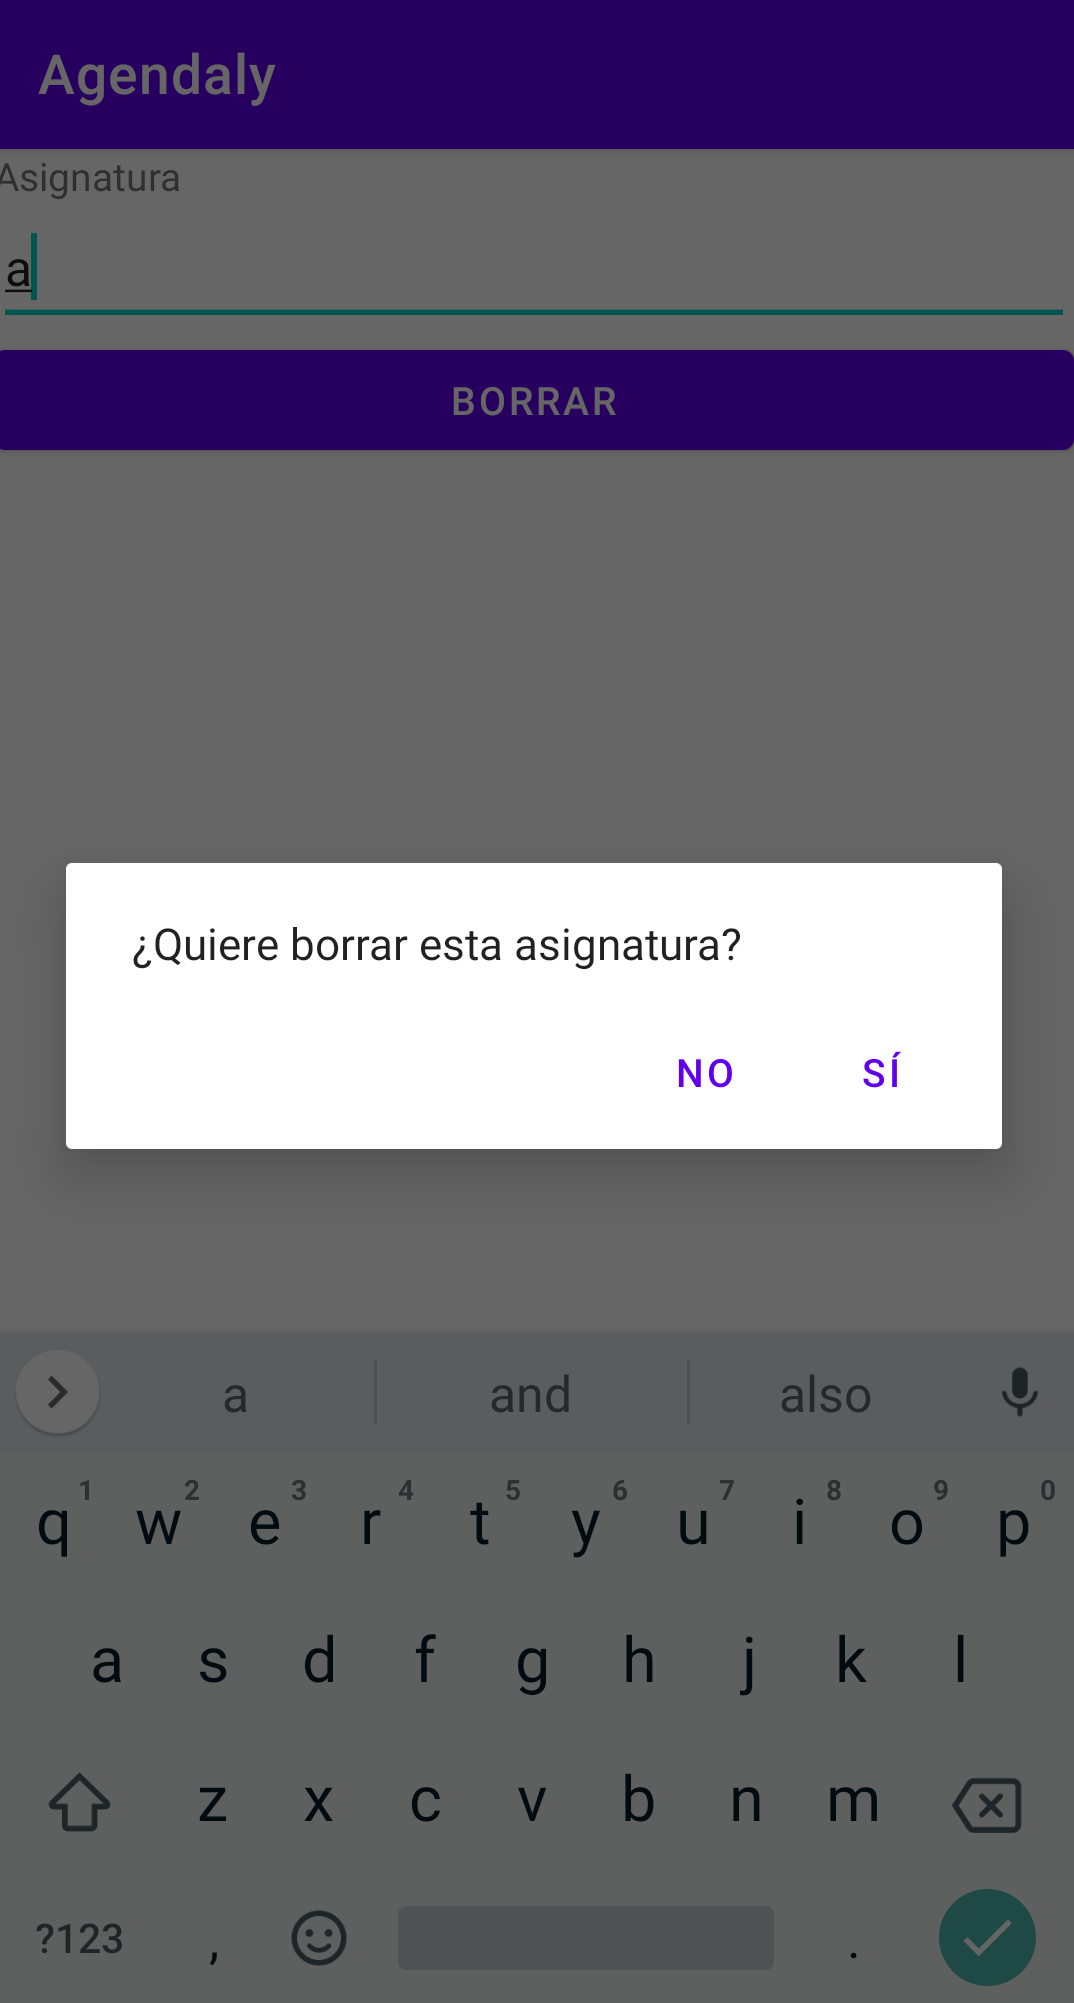
\includegraphics[scale=0.05]{avisoBorr.png}
              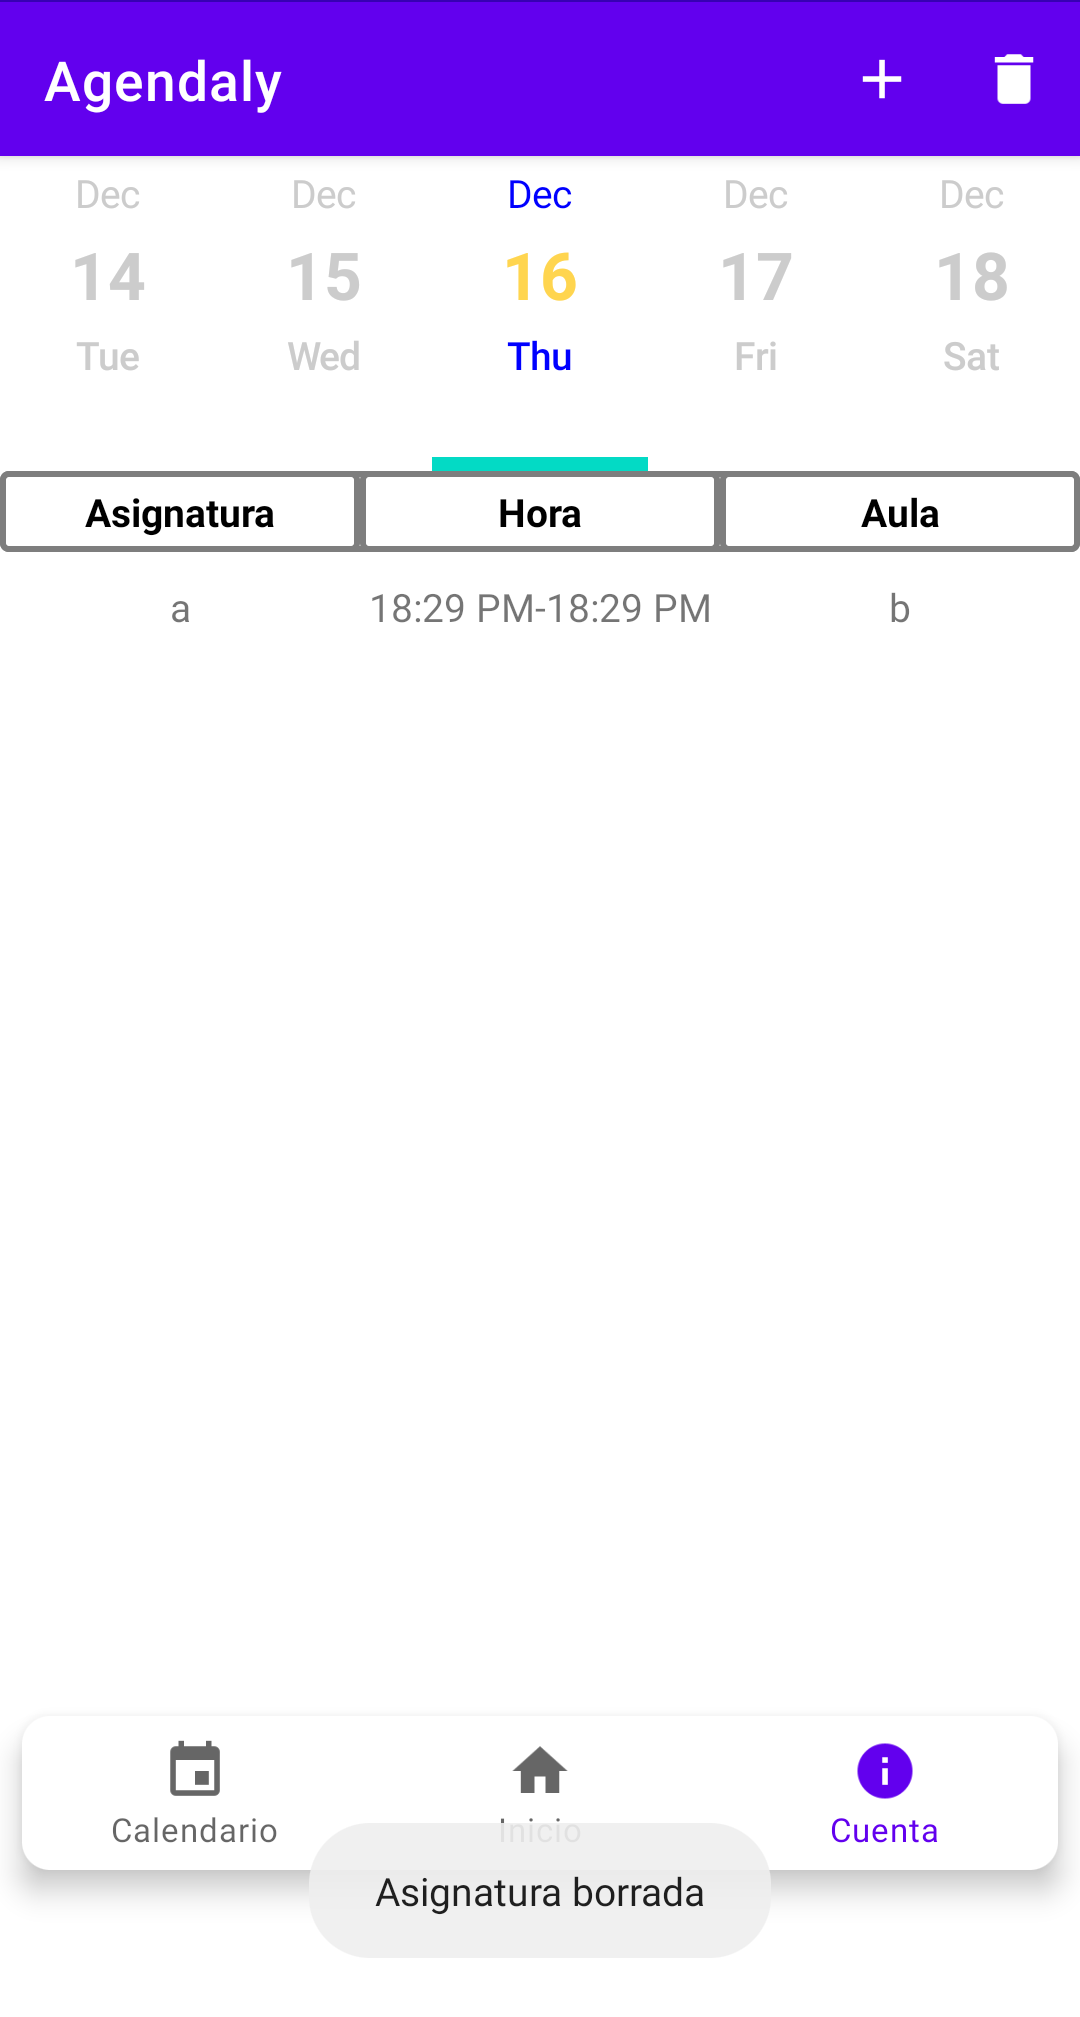
\includegraphics[scale=0.05]{asignaturaBorrToast.png}
            \caption{Pantallas del horario}
        \end{figure}
        
\begin{figure}
            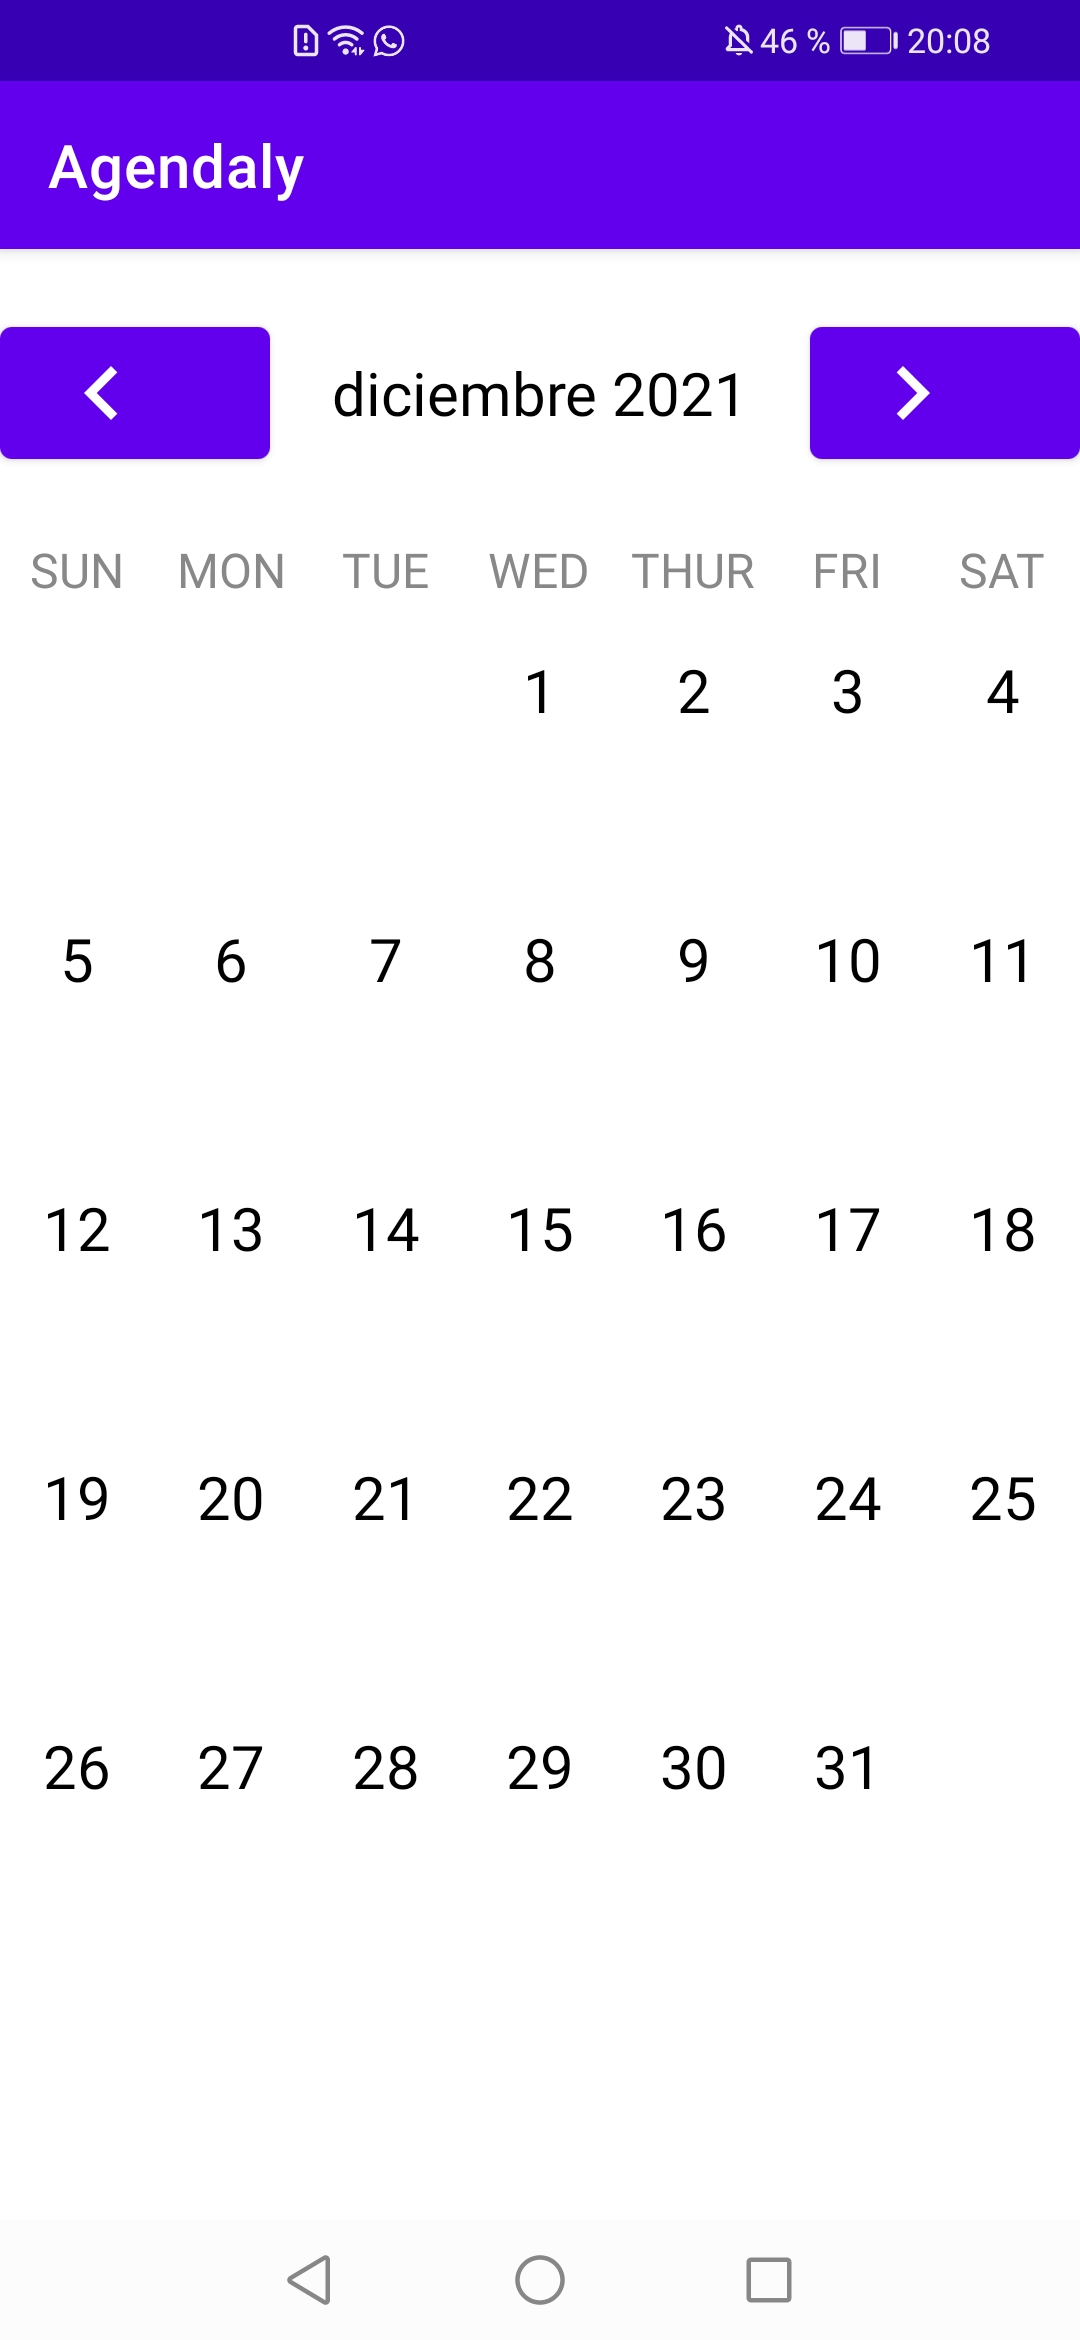
\includegraphics[scale=0.05]{calendarinitview.jpg} \hfill
            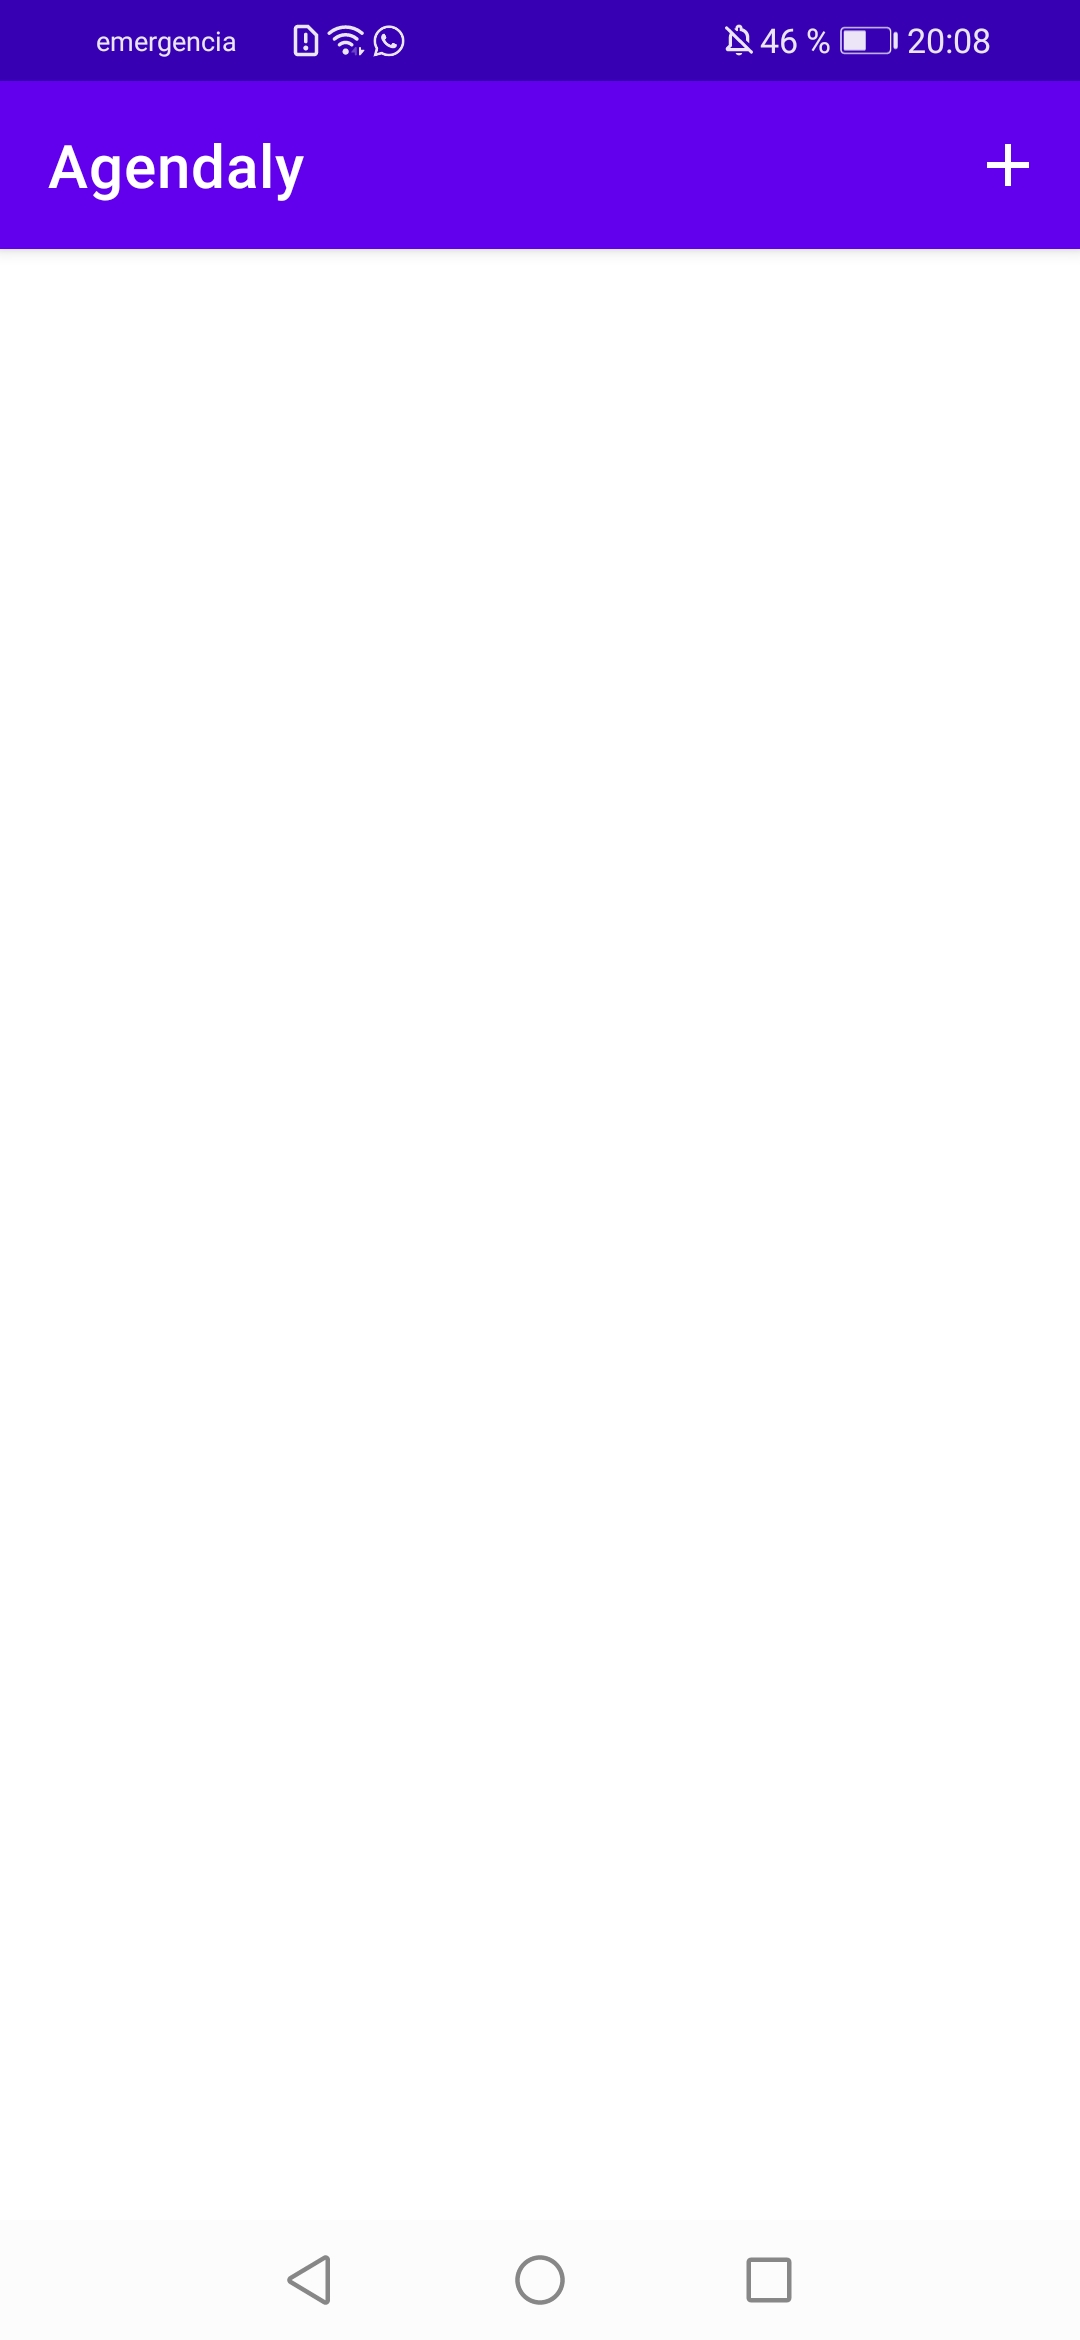
\includegraphics[scale=0.05]{selectedemptyday.jpg}\hfill
            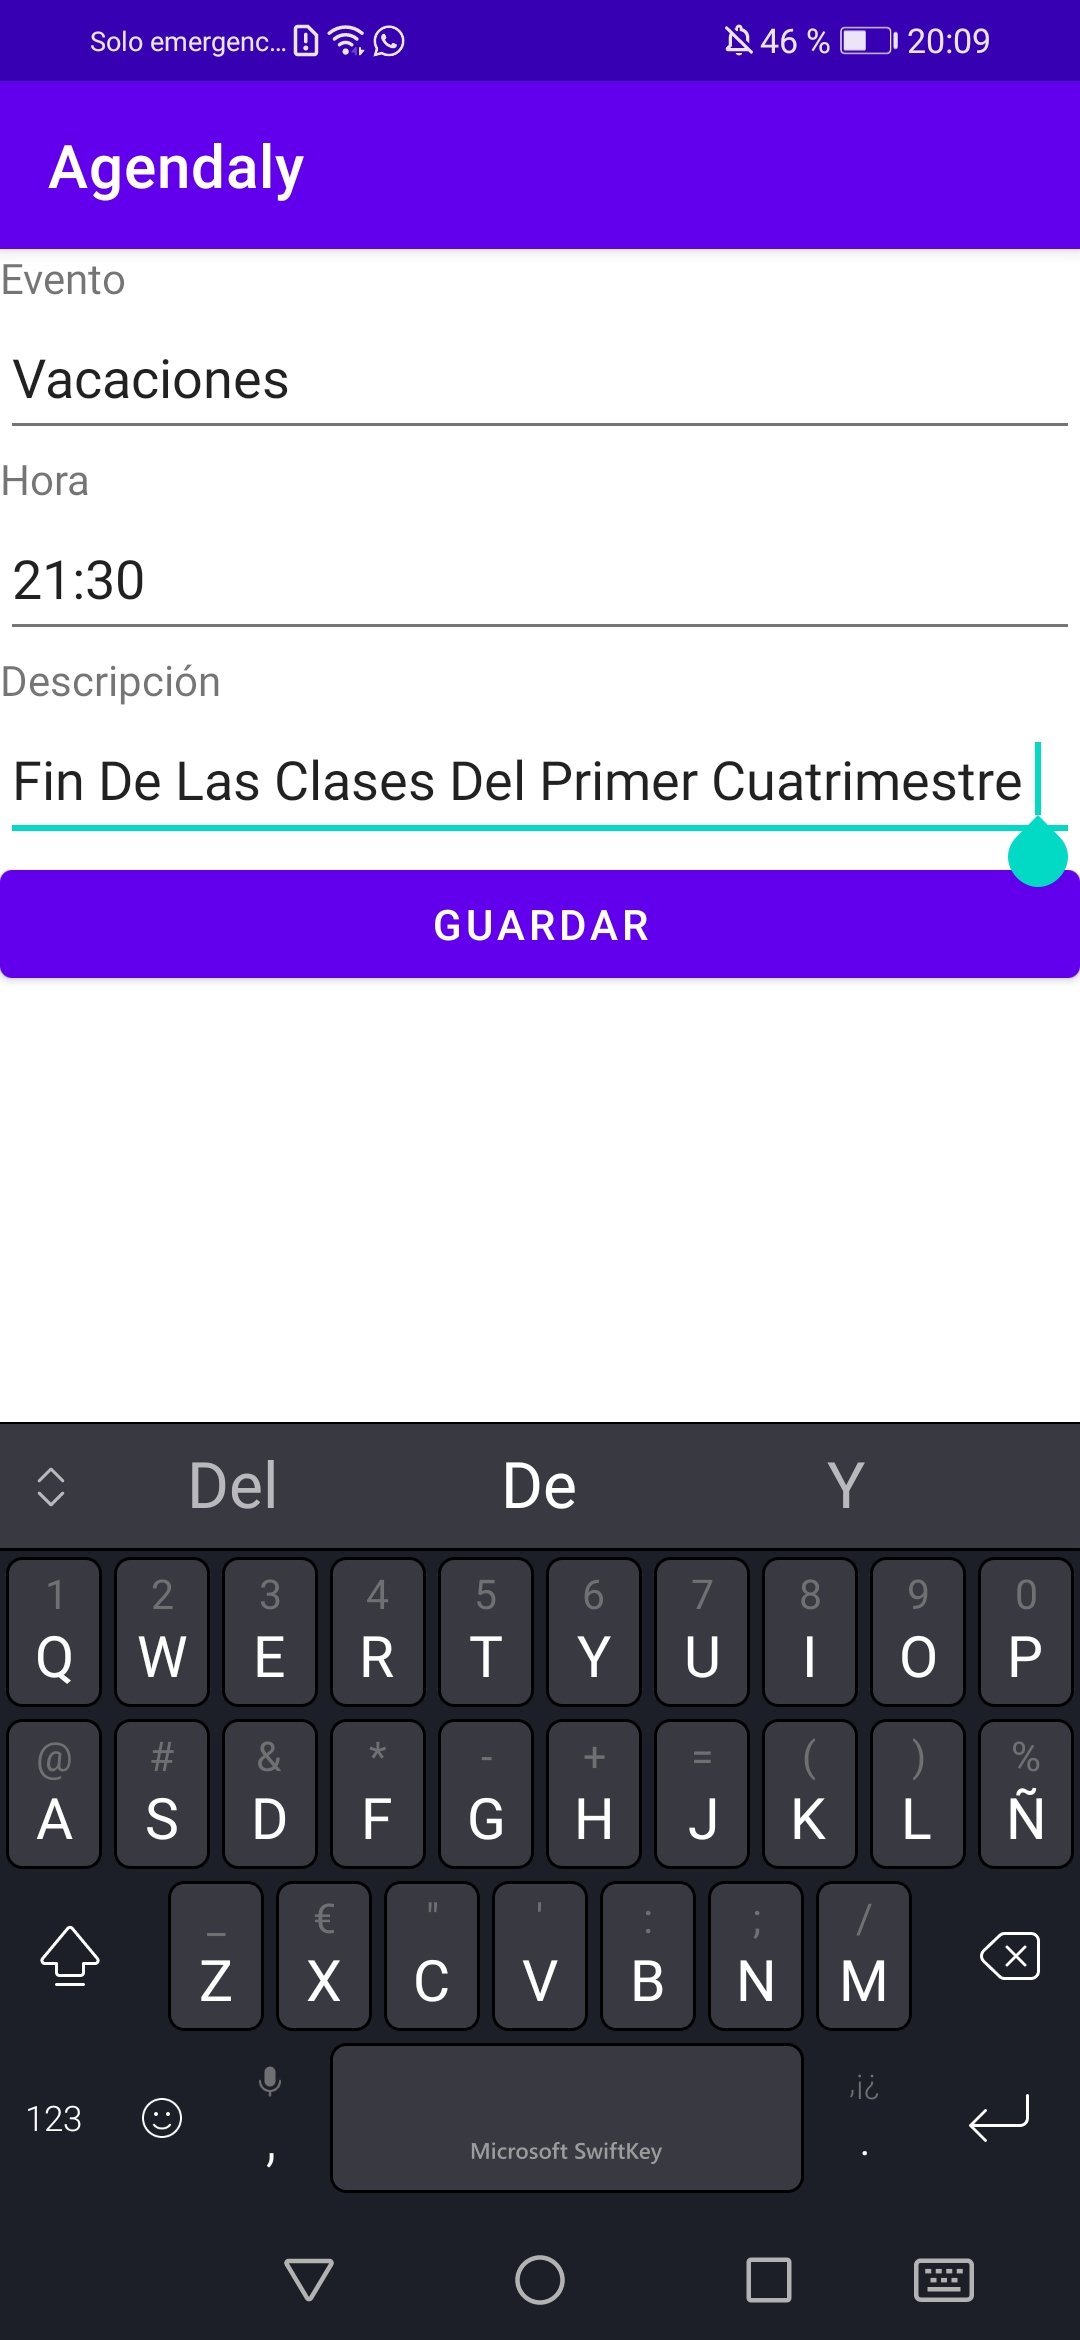
\includegraphics[scale=0.05]{addevent.jpg} \hfill
            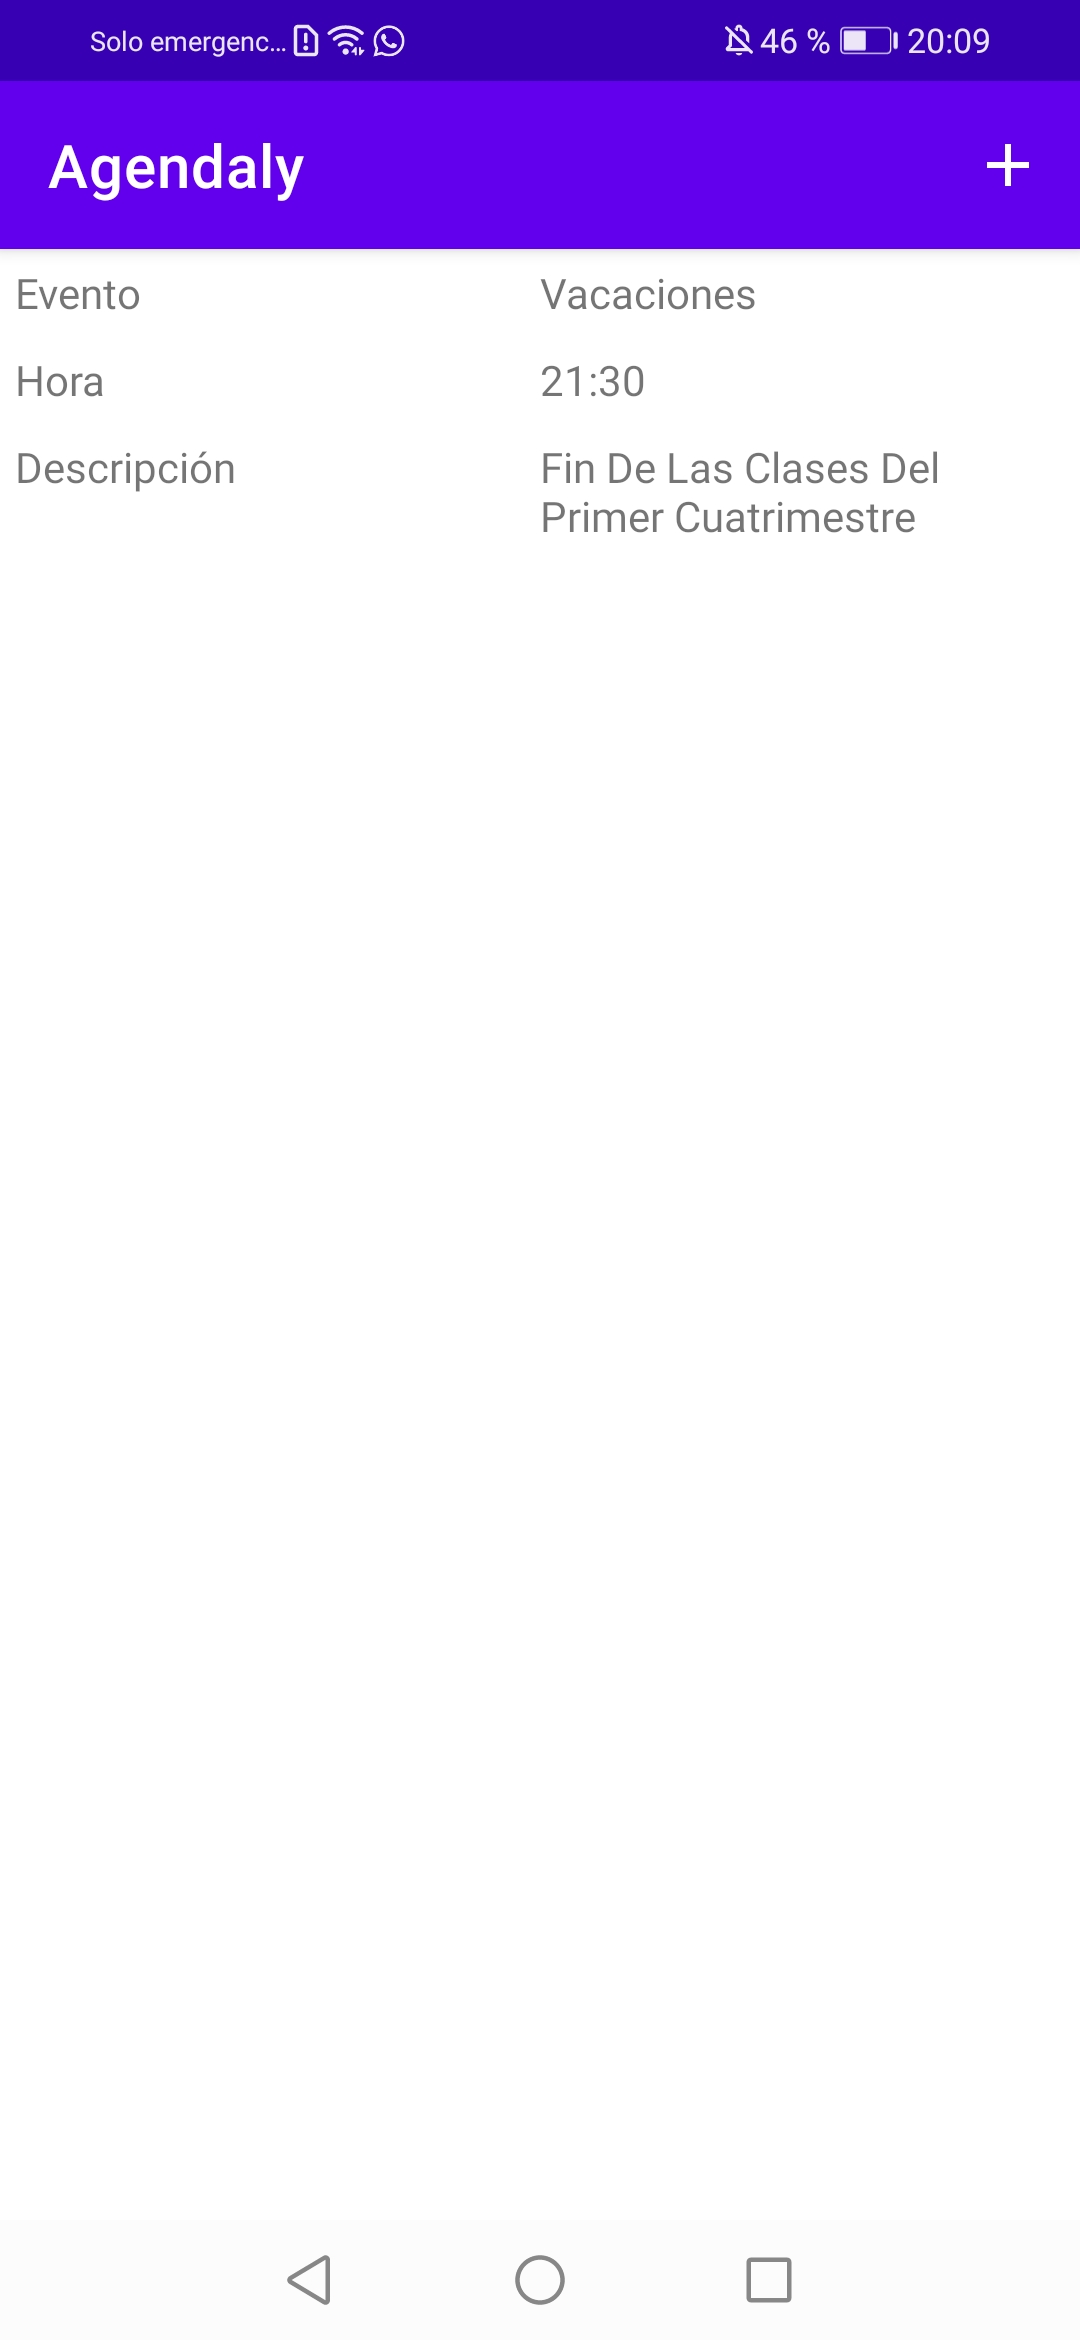
\includegraphics[scale=0.05]{savedevent.jpg}\hfill
            \caption{Pantallas del calendario}
        \end{figure}

\subsection{Comunicaciones}
Necesitamos comunicaciones con servidores para la manutención de usuarios. También necesitaremos un proveedor de bases de datos y comunicación con la API de Google para el calendario.
\subsection{Sensores}
No aplica.
\subsection{Trabajo en background}
Sincronización de datos, gestión de eventos a efectos de notificación, trabajo con bases de datos.

\section{Detalles de la implementación}
Estos se dividirán por tareas:
\begin{itemize}
    \item \textbf{Autenticación}: consta de dos actividades. La actividad AuthenticationActivity y ProfileActivity. En la primera se realiza el log in y el registro, y en la segunda el logout. Al iniciar la aplicación se intenta acceder automáticamente a partir de un fichero de SharedPreferences. Si el fichero está vacío, se le pide al usuario que se registre o inicie sesión. El registro sólo es posible si se usa una cuenta de Agendaly, mientras que si se utiliza Google el inicio de sesión está automáticamente linkado con Firebase. Una vez se realiza este proceso, se lanza la actividad Horario. 
    \newline
    Para el logout, se accede a la pestaña "Cuenta". En esa actividad se muestra información del usuario y un botón para hacer el logout. El proceso de logout es muy simple y funciona con y sin conexión, pues borra los datos locales de acceso, y ejecuta la activity AuthenticationActivity, volviendo a inicial el ciclo de funcionamiento de la aplicación.
    \newline
    En cuanto a la seguridad, la clase AuthUtils abstrae el manejo de usuarios y contraseñas locales, encargándose de guardar, eliminar y obtener datos de usuarios, así como de encriptar las contraseñas. Las contraseñas se guardan encriptadas para que no se puedan obtener manualmente mediante el sistema de ficheros de Android (en caso de dispositivos root o con USB Debug activado).
        
\end{itemize}

\begin{itemize}
    \item \textbf{Horario}: para implementar el horario se usan dos fragmentos y un bottom app bar. \newline
    El bottom appbar nos permite navegar entre el horario, el calendario y la información de usuario autentificado. \newline
    El primer fragmento nos muestra un calendario y el segundo el horario programado para ese día.
    Para el calendario se usa horizontal calendar\cite{misc-hc} que nos permite elegir el día y si mantenemos pulsado una fecha nos lleva al calendario general. \newline
    El segundo fragmento está formado por un Swipe, un TableLayout y un RecyclerView. El Swipe se usa para refrescar el recyclerView en el caso de que hayamos agregado o eliminado una asignatura y no cambiemos de día. El TableLayout nos explica la información que sale por el recyclerView. \newline 
    Las asignaturas se guardan en un base de datos, implementada con Room, guardando de ellas un id generado automáticamente, el nombre de la asignatura, el aula, el día, cuando empieza y cuando acaba. \newline
    Para añadir o eliminar asignaturas se usa un menu formado por dos iconos el + para añadir y un cubo de basura para borrar la asignatura.\newline
    En el momento de añadir una asignatura tendremos que rellenar dos EditText uno con el nombre de la asignatura y otro con el aula, elegir las horas de inicio y fin con un TimePicker para cada uno y por último seleccionar el día de la semana en un Spinner. Una vez cubierto le damos al botón que dice guardar y este guardará esta información en la base de datos local a la vez que nos muestra un Toast que nos dice que se ha guardado correctamente la asignatura.
    \newline
    A la hora de eliminar, tenemos que escribir en un EditText la asignatura a borrar y darle al botón que dice borrar. En ese momento saldrá un aviso para confirmar que vamos a borrar la asignatura mediante un cuadro de diálogo. Una vez aceptamos borraremos la asignatura de la base de datos local y sacará un Toast confirmando la operación.
    

\end{itemize}

\begin{itemize}
    \item \textbf{Calendario}:
    para el calendario se han creado inicialmente un LinearLayout con los botones de adelante y atrás y el nombre del mes, otro con los nombres de los días de la semana y un RecycledView donde irán los números de cada dia del mes. Las fechas se organizan en seis filas y siete columnas dado que, en el peor de los casos (cuando un mes de 30 o 31 días comienza en fin de semana), puede ser necesario utilizar las seis filas para representar todos los días del mes. Cada celda contiene únicamente el número del día que representa.  Cuando se selecciona un día del mes, se lanza una nueva actividad que muestra los eventos planeados para ese día, cada uno en forma de 3 textos: el título del evento, la hora a la que va a tener lugar y una breve descripcion del mismo. Para obtener los valores de estos campos para cada evento, se accede a la base de datos implementada en Room. En esta actividad también existe un menú que permite añadir nuevos eventos. Si se selecciona, se lanzará una nueva actividad con tres textos que se corresponden con los campos qe almacena cada evento y un EditText por cada uno, para que los datos con los que se rellenen sean aquellos que se añaden a la base de datos para cada evento. Cuando se acaben de especificar estos campos, existe el botón de guardar, que añade el evento y los atributos introducidos a la base de datos. Por último, se mostrará un Toast en la parte inferior que verifica que el evento ha sido añadido correctamente.
\end{itemize}

%%%%%%%
%%%%%%%




\bibliographystyle{pfc-fic}
\bibliography{biblio}
\addcontentsline{toc}{section}{Bibliografía}

\end{document}
